\documentclass[11pt, a4paper, oneside]{Thesis}
\graphicspath{{./Figures/}}

\usepackage[square, numbers, comma, sort&compress]{natbib} 
\usepackage{array, booktabs, multirow, longtable}
\usepackage{listings}
\usepackage{color}
\usepackage{blindtext}
\usepackage{tabularx}
\usepackage{makecell, amsmath, amssymb}
\usepackage{tikz, bookmark, tcolorbox, qtree, tikz-qtree}
\usepackage{algorithm}
\usepackage{algorithmic}

%\usepackage{algpseudocode}

\usetikzlibrary{shapes.geometric, arrows}
\usepackage[x11names]{xcolor}
\usetikzlibrary{positioning, shapes, arrows.meta,decorations.pathmorphing}

\definecolor{dkgreen}{rgb}{0,0.6,0}
\definecolor{gray}{rgb}{0.5,0.5,0.5}
\definecolor{mauve}{rgb}{0.58,0,0.82}

\lstset{frame=tb,
  language=Java,
  aboveskip=3mm,
  belowskip=3mm,
  showstringspaces=false,
  columns=flexible,
  basicstyle={\small\ttfamily},
  numbers=none,
  numberstyle=\tiny\color{gray},
  keywordstyle=\color{blue},
  commentstyle=\color{dkgreen},
  stringstyle=\color{mauve},
  breaklines=true,
  breakatwhitespace=true,
  tabsize=3
}

\newcommand{\todo}[1]{\textcolor{red}{(TODO) #1}}
\hypersetup{urlcolor=black, colorlinks=true}
\title{\ttitle} % Defines the thesis title - don't touch this
\begin{document}
\frontmatter
\setstretch{1.3} % Line spacing of 1.3
\fancyhead{} % Clears all page headers and footers
\rhead{\thepage} % Sets the right side header to show the page number
\lhead{} % Clears the left side page header
\pagestyle{fancy} % Finally, use the "fancy" page style to implement the FancyHdr headers



\newcommand{\HRule}{\rule{\linewidth}{0.5mm}} % New command to make the lines in the title page
\hypersetup{pdftitle={\ttitle}}
\hypersetup{pdfsubject=\subjectname}
\hypersetup{pdfauthor=\authornames}
\hypersetup{pdfkeywords=\keywordnames}


%-----------------
%	FIRST PAGES
%-----------------

\begin{titlepage}
    \begin{center}

        \begin{figure}[htbp]
            \centering
            \includegraphics[width=0.24\textwidth]{LU.jpg}
        \end{figure}

        \textsc{\LARGE Lancaster University}\\[0.7cm]
        \HRule \\[0.7cm]
        {\huge \textit{A Monte Carlo Tree Search for the Optimisation of Flight Connections}}\\[0.4cm]
        \HRule \\[0.7cm]
        {\LARGE \bfseries Arnaud Da Silva}\\[0.4cm]
        {\LARGE  36471977}\\[1cm]
        {\large  \bfseries Supervisor }\\[0.4cm]
        {\large \bfseries Ahmed Kheiri}\\[1cm]
        \large \textit{A thesis submitted in fulfillment of the requirements\\ for the degree of Master of Science Business Analytics}\\[0.3cm] % University requirement text
        \textit{in the}\\[0.4cm]
        Lancaster University Management School \\
        Department of Management Science\\[1cm] % Research group name and department name
        {\large September 2024}\\[4cm]
        \vfill
    \end{center}
\end{titlepage}



\Declaration{

    \addtocontents{toc}{\vspace{1em}}  % Add a gap in the Contents, for aesthetics

    I, \textbf{Arnaud Da Silva}, hereby declare that this thesis entitled, \textbf{A Monte Carlo Tree Search for the Optimisation of Flight Connections}, is all my own work, except as indicated in the text.

    The report has been not accepted for any degree and it is not being submitted currently in candidature for any degree or other reward.



    Signed:\\
    \rule[1em]{25em}{0.5pt}  % This prints a line for the signature

    Date:\\
    \rule[1em]{25em}{0.5pt}  % This prints a line to write the date
}
\clearpage  % Declaration ended, now start a new page

%% ----------------------------------------------------------------





\addtotoc{Abstract}

\abstract{\addtocontents{toc}{\vspace{1em}}

    %    \todo{Give a short (1 page) overview of the work. This should summarise (not advertise) your research project. After reading the abstract the reader should know what problem you are tackling, the techniques you are using, the results you have achieved.}
}

Kiwi.com has proposed a real-world NP-hard optimisation problem, focused on air transport services, which involves determining the cheapest connection between specific zones. Despite some similarities with the classic TSP problem, the problem is more complex. It is an asymmetric, time-constrained and generalised (i.e. it involves zones that contain sets of cities, only one of which is visited) TSP. In addition, infeasibility adds further complexity to the problem as there are no flights available between specific points in the network on certain days. Exact methods often fail in solving these computationally difficult problems, particularly as the size of the problem instance increases; alternative approaches, such as heuristics, are therefore preferred in solving the problems.

To tackle this challenge, we implemented a Monte Carlo Tree Search (MCTS), a tree search algorithm typically used in board games. We adapted and tuned it with various parameters and functions, successfully solving six out of eight instances and establishing a new state-of-the-art solution.

\clearpage


\setstretch{1.3}

\acknowledgements{\addtocontents{toc}{\vspace{1em}}

I would like to particularly thanks Ahmed Kheiri, my tutor, who guided me throughout
this work. I would also like to express my gratitude to Yaroslav Pylyavskyy for his
valuable insights and feedbacks on this project. Finally, I would like to thank the
Management Science Department at Lancaster University who have taught me a lot
during this final year of my studies.

}
\clearpage


%-------------------------------------------
%	LIST OF CONTENTS/FIGURES/TABLES PAGES
%-------------------------------------------

\pagestyle{fancy} % The page style headers have been "empty" all this time, now use the "fancy" headers as defined before to bring them back
\lhead{\emph{Contents}} % Set the left side page header to "Contents"
\tableofcontents % Write out the Table of Contents
\lhead{\emph{List of Figures}} % Set the left side page header to "List of Figures"
\listoffigures % Write out the List of Figures
\lhead{\emph{List of Tables}} % Set the left side page header to "List of Tables"
\listoftables % Write out the List of Tables


%-----------------
%   ABBREVIATIONS
%-----------------

\input{First_Pages/abbreviations}
\input{First_Pages/dedication}

%-----------------
%	CHAPTERS
%-----------------

\mainmatter % Begin numeric (1,2,3...) page numbering
\pagestyle{fancy} % Return the page headers back to the "fancy" style
\chapter{Introduction}
\label{Chapter1}
\lhead{Chapter 1. \emph{Introduction}}

%\todo{Set the scenes. Explain why you are doing this work and why the problem being solved is difficult. Most importantly you should clearly explain what the aims and objectives of your work are.}

%\todo{Structure of the thesis. Academic publications produced (if any), including any achievements/highlights}

\section{Background}

The number of flight connections keep increasing every year \cite{statista_flights_year}, more than 38 million flights have been scheduled in 2023 - therefore, creating a challenge for traveler's to find the best and cheapest flight connections for their specific journey, especially when one has to visit a big number of cities.
Consequently, travel agencies have deployed online trip planner algorithms in order to find flights connection that match the traveler's requirements. Example of these are, Google Flights, OpenFlights.org, Skyscanner, Kayak and Kiwi.com.

These agencies have launched different challenges to create and build powerful trip planner algorithms. For instance, as mentionned in \cite{reinforcement_learning_yaro}, OpenFlights.org launched the Air Travelling Salesman project. Furthermore, Kiwi.com has launched a project in 2017, called Traveling Salesman Challenge, where the current algorithm used by Kiwi.com was developed. In 2018, Kiwi.com launched a new challenge, the Traveling Salesman Problem 2.0 which is the focus of this study.

The given problem is a variant of the Traveling Salesman Problem. It can be characteristed as a generalised, assymetric and time dependant TSP.
A traveler has to visit a list of areas, one per day, given a starting airport and all the possible flight connections between these areas at different days. The goal is to determine what is the cheapest flights connection for the traveler to come back to the starting area. Regarding the number of possible journeys, solving this problem by exploring every single potential solution is impossible. This is why a heuristic approach is often used to solve such TSP problem. In this paper, the Kiwi.com challenge is solved using a Monte Carlo Tree Search.
\section{Research objectives}
\label{section:research_obj}
The goals of this dissertation are:
\begin{itemize}
    \item The implementation of a Python innovative solution to solve the Kiwi.com Traveling Salesman problem 2.0 with no focus on the time limit.
    \item Focus on instances ($I_1,\ldots I_8$) that represent more realistic scenarios.
    \item Try to find better solutions than the state of the art for the considered instances.

\end{itemize}

\section{Academic publication}
\begin{itemize}
    \item International Conference on Computer, Control, Electrical, and Electronics Engineering (ICCCEEE)
\end{itemize}

\section{Dissertation structure}

The dissertation is structured as follow:
\begin{itemize}
    \item Section \ref{Chapter2} is the litterature review where the Air Travel optimisations problem are introduced, TSP and its variants are redefined and finally the Monte Carlo Tree Search and an example are presented.
    \item Section \ref{Chapter3} is the problem and instances description to highlight the problem complexity in detail.
    \item Section \ref{Chapter4} is the methodology of our algorithm implementation, where we explain the code's structure, explain the general flow of the algorithm.
    \item Section \ref{Chapter5} is the result and performance of our implementation compared to the state of the art solution and further analysises regarding the MCTS' parameters.
\end{itemize}


\chapter{Literature Review}
\label{Chapter2}
\lhead{Chapter 2. \emph{Literature Review}}
\todo{Present a survey of your main approach and an overview of the approaches proposed previously for solving the problem dealt with in this work}

\todo{Identify the practical and research motivation of this work and the literature gaps}

\todo{How convincing is the authors' argument? (Critical response - comparisons with other research, strengths or weaknesses but in relation to your research)}
\section{Optimisation in Air Travel}

In this section, we discuss some common challenges faced by airline companies and demonstrate the importance of optimisation in decision-making. The goal is to provide insight into some important optimisation problems, underscoring their importance for the success and competitiveness of airline companies.

\subsection{Fleet Assignment Problem}


The Fleet Assignment Problem (FAP), as discussed in \cite{airline_fleet_assignement} involves assigning different types of aircraft, each with specific capacities, to flights based on their capabilities, operational costs, and revenue potential. This decision greatly influences airline revenues and is a vital part of the overall scheduling process. The complexity of FAP is driven by the large number of flights an airline manages daily and its interdependencies with other processes like maintenance and crew scheduling.


\subsection{Crew Scheduling Problem} % (fold)

The Crew Scheduling Problem (CSP), as discussed in \cite{crew_scheduling_problem}, involves assigning crews to a sequence of tasks, each with defined start and end times, with the primary objective of ensuring that all tasks are covered while adhering to regulations on maximum working hours for crew members.

This problem is particularly critical for low-cost carriers, for instance in the United Kingdom in 2023, the low-cost carriers comprise 48\% of the scheduled capacity (total number of seats offered) \cite{lcc_new_norm}, which rely heavily on optimised crew schedules to maintain competitiveness. Efficient crew scheduling is essential not only for low cost carriers and for cost minimisation but also for ensuring operational reliability and flexibility in response to unexpected disruptions.  \cite{ryanair_youtube_report}


\subsection{Disruption Management} % (fold)
\label{sub:disruption management}

Disruptions in airline operations, as noted in \cite{disruption_management}, can occur due to various factors, including crew unavailability, delays from air traffic control, weather conditions, or mechanical failures. Given that flight schedules are typically planned months in advance \cite{flight_scheduling}, effective disruption management is crucial to minimise the impact on passengers and overall airline operations.

The two mains drivers of disruption management are aircraft and crew recovery.
\begin{itemize}
    \item Aircraft recovery: Reassigning aircraft to flights after disruption by taking care of schedules, airports availibility and maintenance. Optimisation tools help manage the complex logistics of matching available aircraft with rescheduled flights, considering factors like airport availability and maintenance requirements. This ensures that the revised schedules are as efficient and practical as possible.
    \item Crew recovery: reassigning crew members to flights by respecting all flights are staffed appropriattely. Optimisation tools are used to adjust crew schedules, taking into account factors such as legal working hours, crew availability, and the need to cover all flights efficiently. These tools help in developing feasible and compliant crew rosters that adapt to the new flight schedules.
\end{itemize}

These optimisation strategies, supported by advanced software, for instance \cite{inform_software} and \cite{ibs_software}, are crucial for reducing the impact of disruptions and boosting operational resilience in the airline industry.

\subsection{Airline adaptation to new demand} % (fold)
\label{sub:Airline adaptation to new demand}


Airlines companies must continuously adapt their schedules to meet evolving market demands, particularly with the growing dominance of leisure travel over business travel, which has introduced new patterns of demand seasonality, especially in Europe as shown on Figure \ref{fig:European_demand_seasonality}. This seasonality poses a challenge for airlines as they have to balance high demand during peak seasons with the risk of underutilisation during off-peak times.

\begin{figure}[!ht]
    \centering
    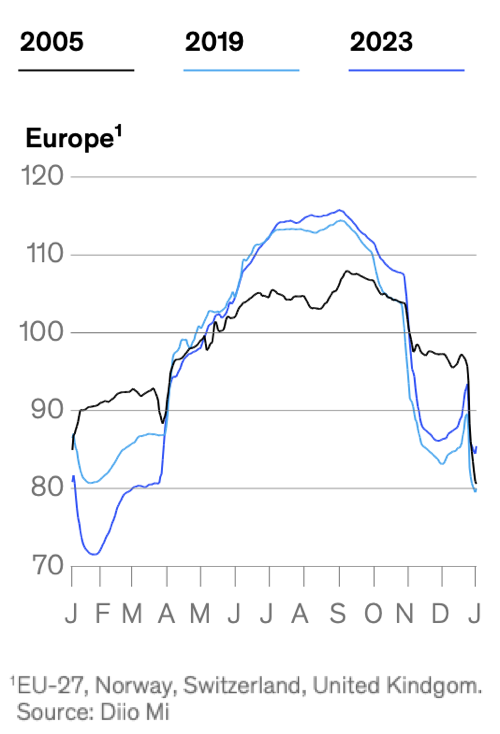
\includegraphics[width=.3\textwidth]{Figures/European Demand.png}
    \caption{European demand seasonality \cite{flight_seasonnality_challenges}}
    \label{fig:European_demand_seasonality}
\end{figure}


Since travel demand varies throughout the year, seasonal-wise, airlines use a variety of techniques to achieve operational efficiency while maximising revenue \cite{flight_seasonnality_challenges}. The seats that airlines book are nearly 65\% more in August than they do in February when summer peak demand skyrocketed. They make the required allowance for additional aircraft and crew by optimisation models that specify priority routes and requirements for additional flights, alongside effective crew rotation management to have everything go smoothly due to the heightened demand of resources.
\\In contrast, winter months pose a different type of problem: demand drops, meaning potential underutilisation of aircraft. To do this, airlines are known to turn to ACMI leasing (agreement between two airlines, where the lessor agrees to provide an aircraft, crew, maintenance and insurance \cite{acmi_def}) during periods of low demand to temporarily reduce fleet size by outsourcing their capacity. Parallel to this, they also increase maintenance activities and incentivise crews to take holidays or undergo training to maximise productivity across the operation. Equally, on a year-round basis, airlines apply dynamic pricing algorithms to vary fares in reaction to real-time demand patterns. In high-demand summer months, fares are tactically set so as to maximise revenues from travelers willing to pay more, while in winter, pricing strategies are aimed at stimulating demand with fare reductions to fill seats that otherwise would have gone empty and improve overall aircraft utilisation. Such adaptive strategies are critical to the airlines for effectively beating the seasonal ebbs and flows in the travel industry.

%\begin{figure}[!ht]
%    \centering
%    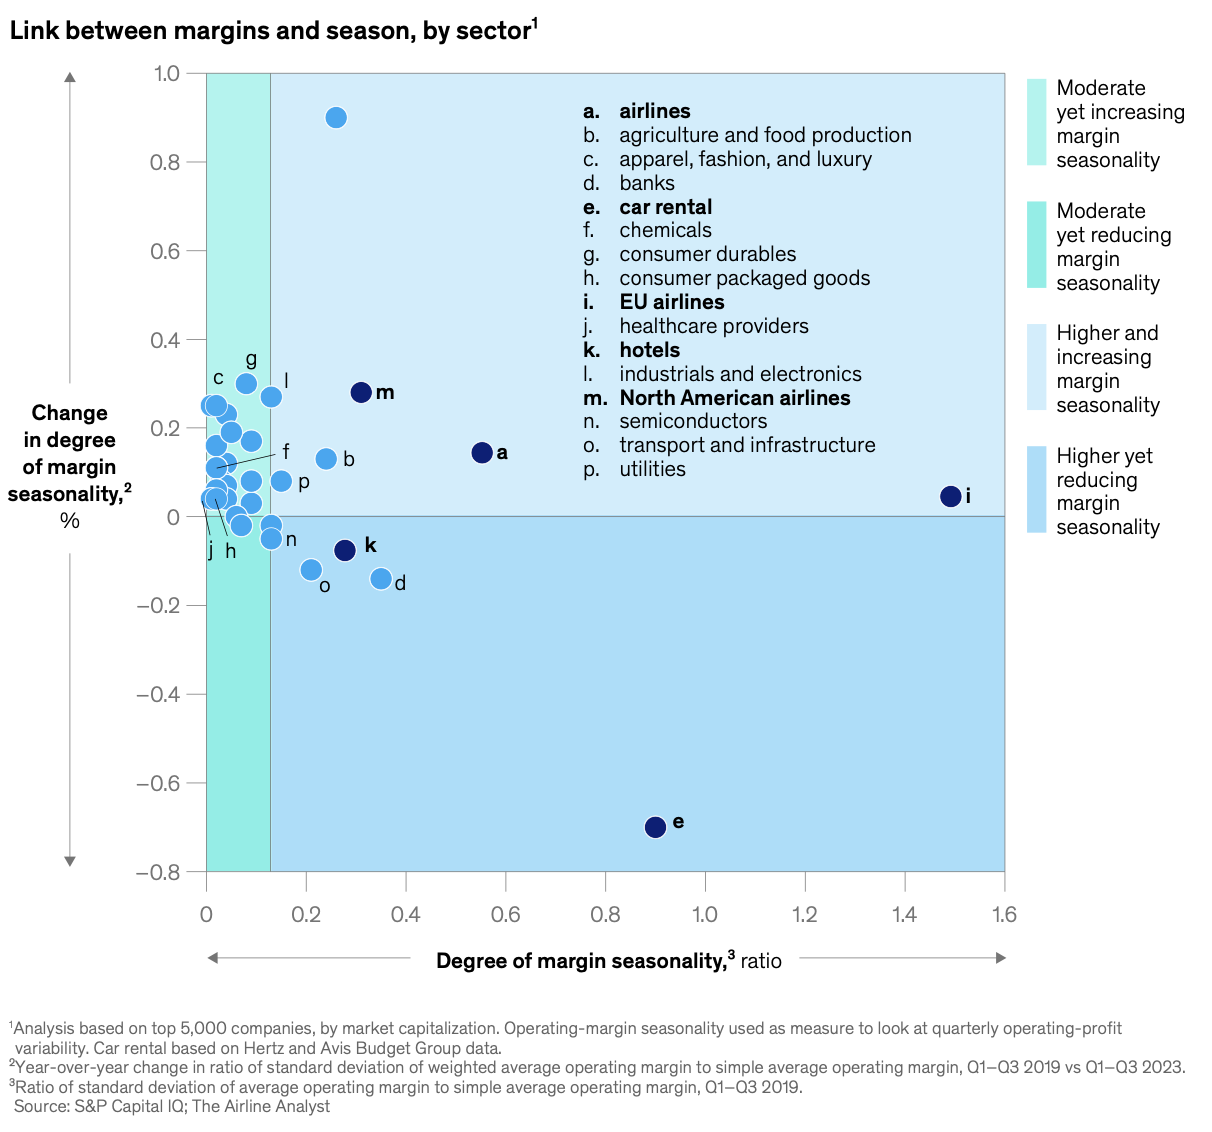
\includegraphics[width=1\textwidth]{Figures/Seasonal margin analysis.png}
%    \caption{Compared with other sectors, airlines exhibit a significant and growing link between margins and seasons.}
%    \label{fig:airline_seasonnality_margin}
%\end{figure}



\newpage
\section{Traveling Salesman problem and its adapation}
\label{sec:TSP}

The Traveling Salesman Problem is a well known problem in the Operational Research and Computer Science area. The basic version of the TSP is to find the best roundtrip for a saleman that has to travel around a given number of cities while minimising the overall journey's distance.
This problem is characterised as $\mathcal{NP}$-Hard \cite{np_hardness}. This means that there is no known polynomial-time algorithm that can solve all instances of the problem efficiently . In terms of time complexity, if we were to solve it explorating all the possible solutions the time complexity would have been $\mathcal{O}(\frac{(n-1)!}{2})$ where $n$ represents the number of cities.

\begin{figure}[!ht]
    \centering
    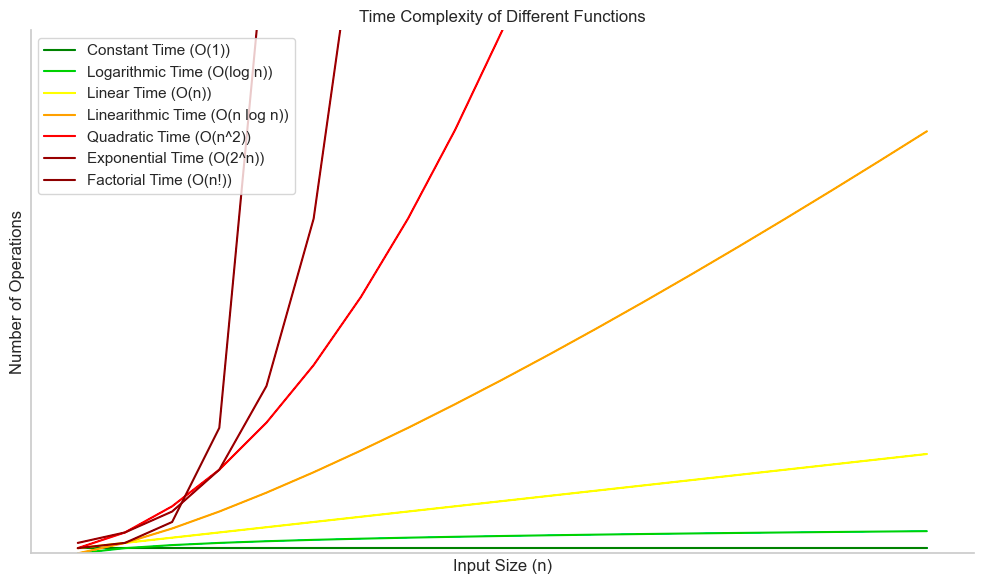
\includegraphics[width=0.8\textwidth]{Figures/NP-hardness - time complexity.png}
    \caption{Time complexity of different functions \cite{time_complexity}}
    \label{fig:time_complexity_comparisons}
\end{figure}

On Figure \ref{fig:time_complexity_comparisons}, different time complexity are compared and the factorial time complexity is the worst. That means that these kinds of $\mathcal{NP}$-Hard problem are typically not solved exploiting all the search area but using heuristics algorithms. Heuristics solutions do not guarantee to find the absolute optimal solution but can find near-optimal solutions in a much more reasonnable times.

The TSP has been studied extensively, not least because many variants can be derived from it:

\begin{itemize}
    \item Symmetric TSP (STSP): The distance between cities are symmetric, meaning that the distance to travel from city A to city B is the same as from city B to city A. %\cite{STSP}
    \item Assymetric TSP (ATSP): The distance between cities are assymetric, meaning that the distance to travel from city A to city B is different than the distance to travel from city B to city A.\cite{ASTP}
    \item Multiple TSP (mTSP): Instead of one salesman, multiple salesman are starting from one city visit all the cities such that each city is visited exactly once. \cite{mTSP}
    \item Time Window TSP (TWTSP): Each city has to be visited in a defined time slot. \cite{TWTSP}
    \item Price-collection TSP (PCTSP): Not all the cities have to be visited, the goal is to to minimise the overall traveler's distance while maximising the price collected earned when visiting a city. \cite{PCTSP}
    \item Stochastic TSP (STSP): The distances between the cities or the cost of travels are stochastic (\i.e random variables) rather than deterministic. \cite{Stochastic_TSP}
    \item Dynamic TSP (DTSP): The problem can change over the times, that means that new cities can be added or distances between cities can change while the salesman has already started his journey. \cite{DTSP}
    \item Generalised TSP (GTSP): The cities are grouped into clusters, the goal is to visit exactly one city from each cluster. \cite{GTSP}
    \item Open TSP (OTSP): The traveler does not have to end his journey at the starting city. \cite{OTSP}
\end{itemize}

Multiple algorithms have been developed to address these TSP variants, we can classify them into two major categories:

\begin{itemize}
    \item \textbf{Exact Algorithms}: These algorithms aim to find the optimal solution to the TSP by exploring all possible routes or by using mathematical techniques to prune the search space efficiently. Examples include:
          \begin{itemize}
              \item \textbf{Branch and Bound}: This method systematically explores the set of all possible solutions, using bounds to eliminate parts of the search space that cannot contain the optimal solution. It is often used for smaller instances of TSP due to its computational intensity. \cite{branch_and_bound}
              \item \textbf{Cutting Planes}: This technique adds constraints (or cuts) to the TSP formulation iteratively to remove infeasible solutions and converge to the optimal solution. This approach is particularly effective for symmetric TSPs. \cite{cutting_planes}
              \item \textbf{Dynamic Programming}: Introduced by Bellman, this approach breaks down the TSP into subproblems and solves them recursively, which is highly effective for specific TSP variants, though its complexity grows exponentially. \cite{dynamic_programming_tsp}
          \end{itemize}
    \item \textbf{Approximation and Heuristic Algorithms}: These algorithms are designed to find near-optimal solutions within a reasonable time frame, especially for large-scale problems where exact methods are computationally infeasible. Examples include:
          \begin{itemize}
              \item \textbf{Greedy Algorithms}: These algorithms make a series of locally optimal choices in the hope of finding a global optimum. An example is the Nearest Neighbor algorithm, which selects the nearest unvisited city at each step. \cite{greedy}
              \item \textbf{Genetic Algorithms}: Inspired by the process of natural selection, these algorithms evolve a population of solutions over time, using operations such as mutation and crossover to explore the solution space. \cite{genetic_algorithm}
              \item \textbf{Simulated Annealing}: This probabilistic technique searches for a global optimum by allowing moves to worse solutions based on a temperature parameter that gradually decreases. It is particularly useful for escaping local optima. \cite{simulated_annealing}
              \item \textbf{Ant Colony Optimization}: This metaheuristic is inspired by the foraging behavior of ants and uses a combination of deterministic and probabilistic rules to construct solutions, gradually improving them through pheromone updates. \cite{ant_colony}
          \end{itemize}
\end{itemize}

Some TSP problems (or its variants) have been solved using other algorithms, hence they are less traditionnal than those mentionned.

\newpage
\section{The Monte Carlo Tree Search algorithm}

The Monte Carlo Tree Search (MCTS) algorithm can be characterised less traditionnal than the previously enounced method in Section \ref{sec:TSP} to solve TSP because MCTS is typically used in games. MCTS' (and its variants)
have been successfully implemented across a range of games, such as Havannah \cite{wiki:board_game},  Amazons \cite{wiki:Game_of_the_Amazons}, Lines of Actions \cite{wiki:Lines_of_Action}, Go, chess, and Shogi \cite{wiki:Shogi}, establishing it as the state-of-the-art method for many of these games \cite{havannah}, \cite{amazons}, \cite{lines_of_actions}. It is widely use in board games and has been really popular when Google DeepMind developed AlphaGo. AlphaGo is a software that was created to beat the best Go's player in the world.

Go is an ancient board game from China where two players take turns placing black or white stones on a grid. The goal is to capture territory by surrounding empty spaces or the opponent’s stones. Despite its simple rules, Go is incredibly deep and complex, with countless possible moves and strategies. It is known for its balance between intuition and logic, hence it has been a significant focus of artificial intelligence research ,\cite{wiki:Go}. In 2016, Lee Sedol \cite{wiki:Lee_Sedol} - the best Go's player in the world has been beaten by AlphaGo 4-1 \cite{alpha_go_documentary}.

MCTS with policy and value networks are at the heart of AlphaGo's decision-making process, enabling AlphaGo's to pick the optimal moves in the complex search of Go. \cite{mcts_alpha_go_algorithm}



\subsection{Overview}
The MCTS' process is conceptually straightforward. A tree is built in an incremental and assymatric manner (Figure \ref{fig:Assymetrical_growth_MCTS}).
For every iteration, a selection policy is used to determine which node we have to select in the tree to perform simulations.
The selection policy, typically balances the exploration  i.e.\ look into part of the tree that have not been visited yet and the exploitation i.e.\ look into part of the trees that appear to be promising.
Once the node is selected, a simulation i.e.\ a sequence of available actions, based on a simulation policy, are applied from this node until a terminal condition is reached e.g\ no further actions are possible. \cite{mcts_various_policies}

\begin{figure}[!ht]
    \centering
    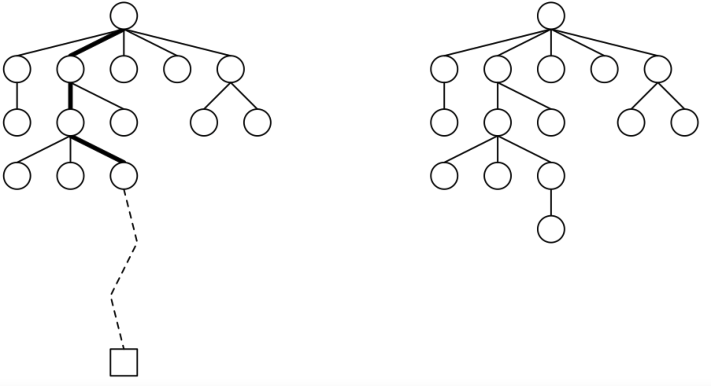
\includegraphics[width=0.5\textwidth]{Figures/assymetric_growth_mcts_tree.png}
    \caption{Assymetrical growth of MCTS - Simulation and Expansion - \cite{mcts_assymetrical_growth}}
    \label{fig:Assymetrical_growth_MCTS}
\end{figure}
To ensure that the reader understands the various stages of the Monte Carlo Tree Search Algorithm, we will begin by looking at a detailed example. This example will illustrate each component of the algorithm in action. We will then generalise the principles discussed, as the basic methodology of this paper is based on the application of the MCTS algorithm.


\subsection{Example}
\label{Example}
Let's say we are given a maximisation problem. When starting the game, you have two possible actions $a_1$ and $a_2$ from the node $S^{0,0}_0$ in the tree $\mathcal{T}$.
Every node is defined like so: $S^{n_i,t_i}_i$ where $n_i$ represents the number of times node $i$ has been visited, $t_i$ the total score of this node.
Furthermore, for every node - we can compute a selection metric, for instance the $UCB1$ value: $UCB1(S^{n_i,t_i}_i)=\bar{V_i} + 2 \sqrt{\frac{\ln N}{n_i}}$ where $\bar{V_i}=\frac{n_i}{t_i}$ represents the average value of the node, $n_i$ the number of times node $i$ has been visited, $N=n_0$ the number of times the root node has been visited (which is also equal to the number of iterations).

Before the first iteration, none node have been visited - $\forall i \in \mathcal{T}, S^{0,0}_{i}$.
\begin{figure}[!ht]
    \centering
    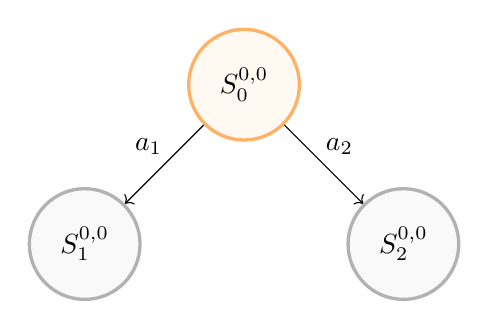
\begin{tikzpicture}[
            root_node/.style={circle, draw=orange!60, fill=orange!5, very thick, minimum size=40},
            visited_node/.style={circle, draw=green!60, fill=green!5, very thick, minimum size=40},
            unvisited_node/.style={circle, draw=gray!60, fill=gray!5, very thick, minimum size=40},
            target_node/.style={circle, draw=green!60, fill=green!5, very thick, minimum size=40},
        ]

        \node[root_node](Root){$S^{0,0}_0$};
        \node[unvisited_node, below left=of Root](S1){$S^{0,0}_1$};
        %\node[target_node, below=of S1, yshift=-1.7cm](Target){};
        \node[unvisited_node, below right=of Root](S2){$S^{0,0}_2$};

        \draw[->] (Root) -- (S1) node[midway, above, xshift=-2mm] {$a_1$};
        \draw[->] (Root) -- (S2) node[midway, above, xshift=2mm] {$a_2$};

        %\draw[->, very thick, decorate, decoration={snake, amplitude=.7mm, segment length=3mm}] (S1) -- (Target);
    \end{tikzpicture}
    \caption{Selection - $I1$}
    \label{fig:Expansion of the tree from the root node}
\end{figure}
At the beginning of $I1$, we then have to choose between these two child nodes (or choose between taking $a_1$ or $a_2$). We then have to calculate the $UCB1$ value for these two nodes and pick the node that maximises the $UCB1$ value (as we are dealing with a maximisation problem).
In Figure \ref{fig:Expansion of the tree from the root node}, neither of these have been visited yet so $USB(S^{0,0}_1)=UCB1(S^{0,0}_2)=\infty$. Hence we decide to choose randomly $S^{0,0}_1$.

$S^{0,0}_1$ is a leaf node that has not been visited - then we can simulate from this node i.e.\ selecting actions from this node based on the simulation policy to a terminal state as shown on Figure \ref{fig:Simulation - $I1$}:

\begin{figure}[!ht]
    \centering
    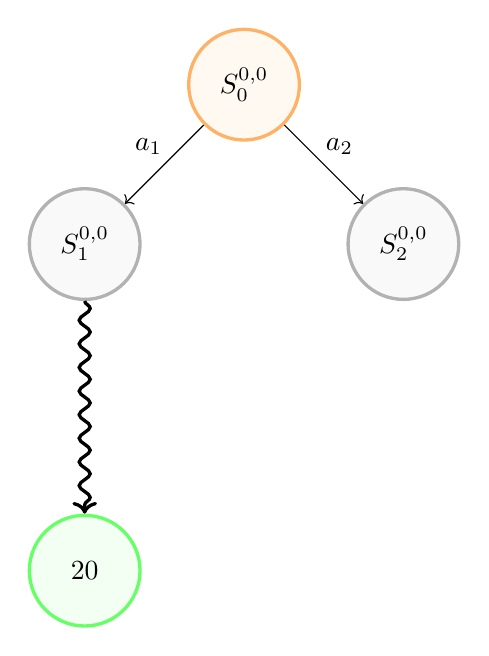
\begin{tikzpicture}[
            root_node/.style={circle, draw=orange!60, fill=orange!5, very thick, minimum size=40},
            visited_node/.style={circle, draw=green!60, fill=green!5, very thick, minimum size=40},
            unvisited_node/.style={circle, draw=gray!60, fill=gray!5, very thick, minimum size=40},
            target_node/.style={circle, draw=green!60, fill=green!5, very thick, minimum size=40},
        ]

        \node[root_node](Root){$S^{0,0}_0$};
        \node[unvisited_node, below left=of Root](S1){$S^{0,0}_1$};
        \node[target_node, below=of S1, yshift=-1.7cm](Target){20};
        \node[unvisited_node, below right=of Root](S2){$S^{0,0}_2$};

        \draw[->] (Root) -- (S1) node[midway, above, xshift=-2mm] {$a_1$};
        \draw[->] (Root) -- (S2) node[midway, above, xshift=2mm] {$a_2$};

        \draw[->, very thick, decorate, decoration={snake, amplitude=.7mm, segment length=3mm}] (S1) -- (Target);
    \end{tikzpicture}
    \caption{Simulation - $I1$}
    \label{fig:Simulation - $I1$}
\end{figure}

\newpage
The terminal state has a value of 20, we can write that the rollout/simulation from node $S^{0,0}_1$ node is $\mathcal{R}(S^{0,0}_1)=20$ . The final step of $I1$ is backpropagation. Every node that has been visited in the iteration is updated.
Let $\mathcal{N}_{\mathcal{R},j}$ be the indexes of the nodes visited during the $j-th$ iteration of the MCTS:
\begin{itemize}
    \item Before backpropagation:
          \begin{equation}
              \forall i \in \mathcal{N}_{\mathcal{R},j}, S^{n_i,t_i}_{i,old}
          \end{equation}

    \item After backpropagation:
          \begin{equation}
              \forall i \in \mathcal{N}_{\mathcal{R},j}, S^{n_i+1,t_i+\mathcal{R}(S^{n_i,t_i}_{i,old})}_{i,new}
          \end{equation}
\end{itemize}

We can then define a backpropagation function:
\begin{center}
    \centering
    $\begin{array}{ccccc}
            \mathcal{B} & : & \mathcal{N}_{\mathcal{R},j} & \to     & \mathcal{N}_{\mathcal{R},j}                    \\
                        &   & S^{n_i,t_i}_{i}             & \mapsto & S^{n_i+1,t_i+\mathcal{R}(S^{n_i,t_i}_{i})}_{i} \\
        \end{array}$
\end{center}



\newpage
Then, back to our example on Figure \ref{fig:Backpropagation_I1} we update the nodes $\mathcal{B}(S^{0,0}_1)=S^{\mathbf{1},\mathbf{20}}_1$ and $\mathcal{B}(S^{0,0}_0)=S^{\mathbf{1},\mathbf{20}}_0$.
\begin{figure}[!ht]
    \centering
    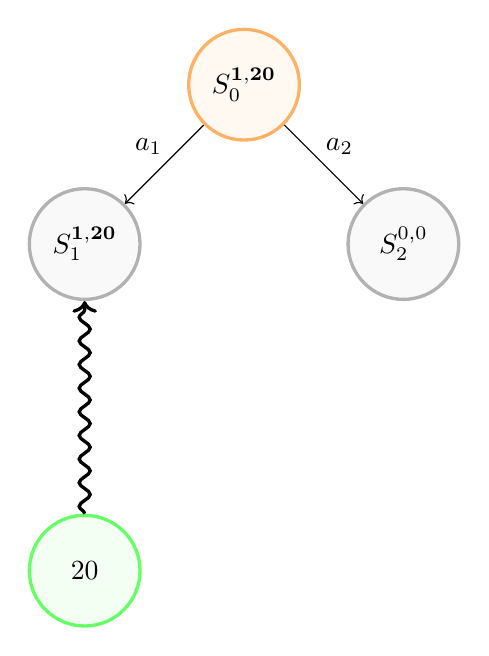
\begin{tikzpicture}[
            root_node/.style={circle, draw=orange!60, fill=orange!5, very thick, minimum size=40},
            visited_node/.style={circle, draw=green!60, fill=green!5, very thick, minimum size=40},
            unvisited_node/.style={circle, draw=gray!60, fill=gray!5, very thick, minimum size=40},
            target_node/.style={circle, draw=green!60, fill=green!5, very thick, minimum size=40}
        ]

        \node[root_node](Root){$S^{\mathbf{1},\mathbf{20}}_0$};
        \node[unvisited_node, below left=of Root](S1){$S^{\mathbf{1},\mathbf{20}}_1$};
        \node[target_node, below=of S1, yshift=-1.7cm](Target){20};
        \node[unvisited_node, below right=of Root](S2){$S^{0,0}_2$};

        \draw[->] (Root) -- (S1) node[midway, above, xshift=-2mm] {$a_1$};
        \draw[->] (Root) -- (S2) node[midway, above, xshift=2mm] {$a_2$};

        \draw[->, very thick, decorate, decoration={snake, amplitude=.7mm, segment length=3mm}] (Target) -- (S1);
    \end{tikzpicture}
    \caption{Backpropagation - I1}
    \label{fig:Backpropagation_I1}
\end{figure}

The fourth phase of the algorithm have been done for $I1$. We can then start the $2^{nd}$ iteration $I2$.
\begin{figure}[!ht]
    \centering
    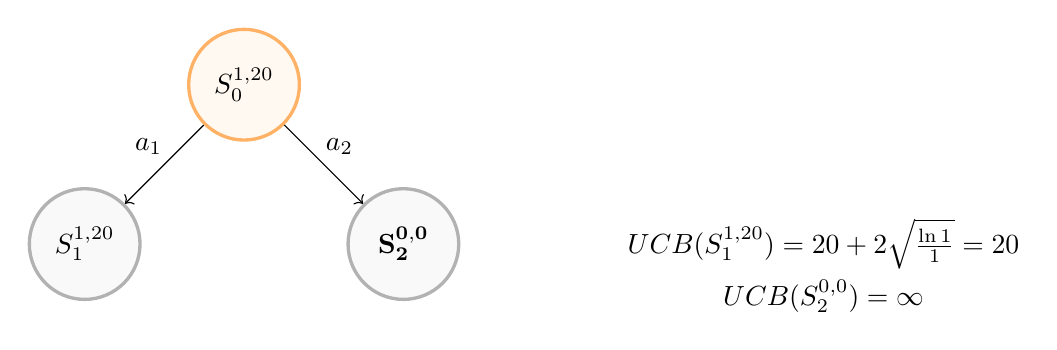
\begin{tikzpicture}[
            root_node/.style={circle, draw=orange!60, fill=orange!5, very thick, minimum size=40},
            visited_node/.style={circle, draw=green!60, fill=green!5, very thick, minimum size=40},
            unvisited_node/.style={circle, draw=gray!60, fill=gray!5, very thick, minimum size=40},
            target_node/.style={circle, draw=green!60, fill=green!5, very thick, minimum size=40}
        ]

        \node[root_node](Root){$S^{1,20}_0$};
        \node[unvisited_node, below left=of Root](S1){$S^{1,20}_1$};
        %\node[target_node, below=of S1, yshift=-1.7cm](Target){20};
        \node[unvisited_node, below right=of Root](S2){$\mathbf{S^{0,0}_2}$};

        \node[right=2cm of S2, anchor=west] (UCB1) {$UCB(S^{1,20}_1)=20+2 \sqrt{\frac{\ln1}{1}} = 20$};
        \node[below=0.55cm of UCB1, anchor=south] (UCB2) {$UCB(S^{0,0}_2)=\infty$};

        \draw[->] (Root) -- (S1) node[midway, above, xshift=-2mm] {$a_1$};
        \draw[->] (Root) -- (S2) node[midway, above, xshift=2mm] {$a_2$};

        %\draw[->, very thick, decorate, decoration={snake, amplitude=.7mm, segment length=3mm}] (S1) -- (Target);
    \end{tikzpicture}
    \caption{Selection - I2}
    \label{fig:Selection - I2}
\end{figure}
On Figure \ref{fig:Selection - I2}, we can either choose $a_1$ or $a_2$. When a child node has not been visited yet, you pick this node for the Selection or you can compute the $UCB1$ value, it leads to the same conclusion.

\begin{figure}[!ht]
    \centering
    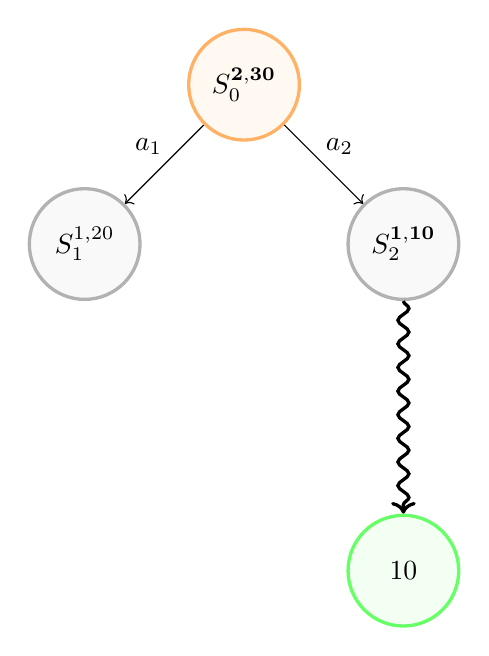
\begin{tikzpicture}[
            root_node/.style={circle, draw=orange!60, fill=orange!5, very thick, minimum size=40},
            visited_node/.style={circle, draw=green!60, fill=green!5, very thick, minimum size=40},
            unvisited_node/.style={circle, draw=gray!60, fill=gray!5, very thick, minimum size=40},
            target_node/.style={circle, draw=green!60, fill=green!5, very thick, minimum size=40},
        ]

        \node[root_node](Root){$S^{\mathbf{2},\mathbf{30}}_0$};
        \node[unvisited_node, below left=of Root](S1){$S^{1,20}_1$};

        \node[unvisited_node, below right=of Root](S2){$S^{\mathbf{1},\mathbf{10}}_2$};
        \node[target_node, below=of S2, yshift=-1.7cm](Target){10};

        \draw[->] (Root) -- (S1) node[midway, above, xshift=-2mm] {$a_1$};
        \draw[->] (Root) -- (S2) node[midway, above, xshift=2mm] {$a_2$};

        \draw[->, very thick, decorate, decoration={snake, amplitude=.7mm, segment length=3mm}] (S2) -- (Target);
    \end{tikzpicture}
    \caption{Simulation and Backpropagation - I2}
    \label{fig:Simulation and Backpropagation - I2}
\end{figure}
\newpage
We can then simulate (Figure \ref{fig:Simulation and Backpropagation - I2}) from the chosen node $S^{0,0}_{2}$ and $\mathcal{R}(S^{0,0}_{2})=10$ and backpropagate all the visited nodes: $\mathcal{B}(S^{0,0}_{2})=S^{1,10}_{2}$ and $\mathcal{B}(S^{1,20}_{0})=S^{2,30}_{0}$.
We now start the $3^{rd}$ iteration, based on the $UCB1$ score we decide to choose $a_1$.
\begin{figure}[!ht]
    \centering
    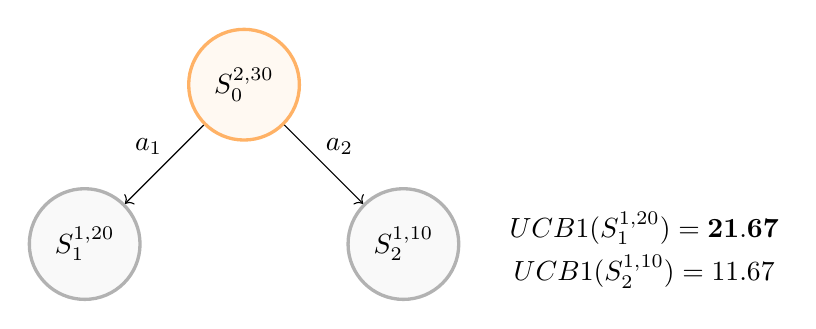
\begin{tikzpicture}[
            root_node/.style={circle, draw=orange!60, fill=orange!5, very thick, minimum size=40},
            visited_node/.style={circle, draw=green!60, fill=green!5, very thick, minimum size=40},
            unvisited_node/.style={circle, draw=gray!60, fill=gray!5, very thick, minimum size=40},
            target_node/.style={circle, draw=green!60, fill=green!5, very thick, minimum size=40},
        ]

        \node[root_node](Root){$S^{2,30}_0$};
        \node[unvisited_node, below left=of Root](S1){$S^{1,20}_1$};

        \node[unvisited_node, below right=of Root](S2){$S^{1,10}_2$};
        %\node[target_node, below=of S2, yshift=-1.7cm](Target){10};
        \node[right=5mm of S2, anchor=west, yshift=2mm] (UCB1) {$UCB1(S^{1,20}_1)=\mathbf{21.67}$};
        \node[below=0.55cm of UCB1, anchor=south] (UCB2) {$UCB1(S^{1,10}_2)=11.67$};

        \draw[->] (Root) -- (S1) node[midway, above, xshift=-2mm] {$a_1$};
        \draw[->] (Root) -- (S2) node[midway, above, xshift=2mm] {$a_2$};

        %\draw[->, very thick, decorate, decoration={snake, amplitude=.7mm, segment length=3mm}] (S2) -- (Target);
    \end{tikzpicture}
    \caption{Selection - I3}
    \label{fig:Selection - I3}
\end{figure}


$S^{1,20}_{1}$ is a leaf node and has been visited so we can expand this node.

\begin{figure}[!ht]
    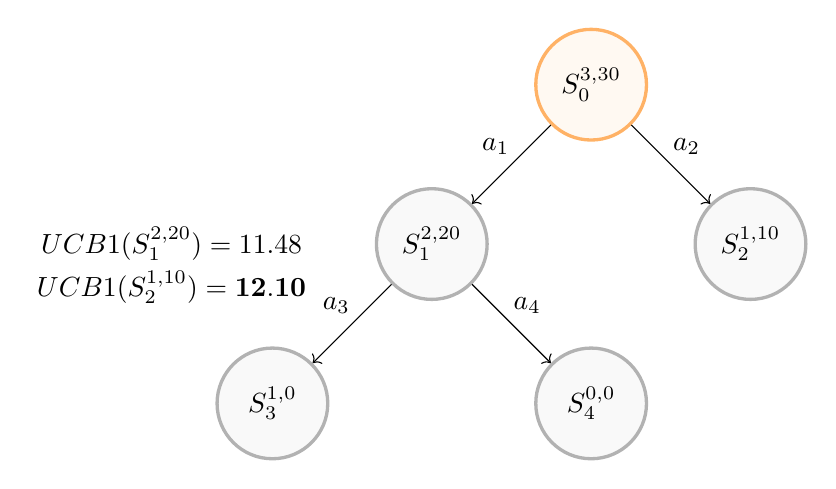
\begin{tikzpicture}[
            root_node/.style={circle, draw=orange!60, fill=orange!5, very thick, minimum size=40},
            visited_node/.style={circle, draw=green!60, fill=green!5, very thick, minimum size=40},
            unvisited_node/.style={circle, draw=gray!60, fill=gray!5, very thick, minimum size=40},
            target_node/.style={circle, draw=green!60, fill=green!5, very thick, minimum size=40},
        ]

        \node[root_node](Root){$S^{3,30}_0$};
        \node[unvisited_node, below left=of Root](S1){$S^{2,20}_1$};
        \node[unvisited_node, below right=of Root](S2){$S^{1,10}_2$};
        \node[unvisited_node, below left=of S1](S3){$S^{1,0}_3$};
        \node[unvisited_node, below right=of S1](S4){$S^{0,0}_4$};

        \node[left=8mm of S1, anchor=east] (UCB1) {$UCB1(S^{2,20}_1)=11.48$};
        \node[below=0.55cm of UCB1, anchor=south] (UCB2) {$UCB1(S^{1,10}_2)=\mathbf{12.10}$};

        %\node[target_node, below=of S3, yshift=-1.7cm](Target){0};

        \draw[->] (Root) -- (S1) node[midway, above, xshift=-2mm] {$a_1$};
        \draw[->] (Root) -- (S2) node[midway, above, xshift=2mm] {$a_2$};
        \draw[->] (S1) -- (S3)   node[midway, above, xshift=-2mm] {$a_3$};
        \draw[->] (S1) -- (S4)   node[midway, above, xshift=2mm] {$a_4$};
        %\draw[->, very thick, decorate, decoration={snake, amplitude=.7mm, segment length=3mm}] (S3) -- (Target);
    \end{tikzpicture}
    \caption{Selection and Expansion - I3}
\end{figure}
\newpage
Based on $UCB1$ score we decide to simulate from $S^{0,0}_3$ on Figure \ref{fig:Simulation and Backpropagation - I3}
\begin{figure}[!ht]
    \centering
    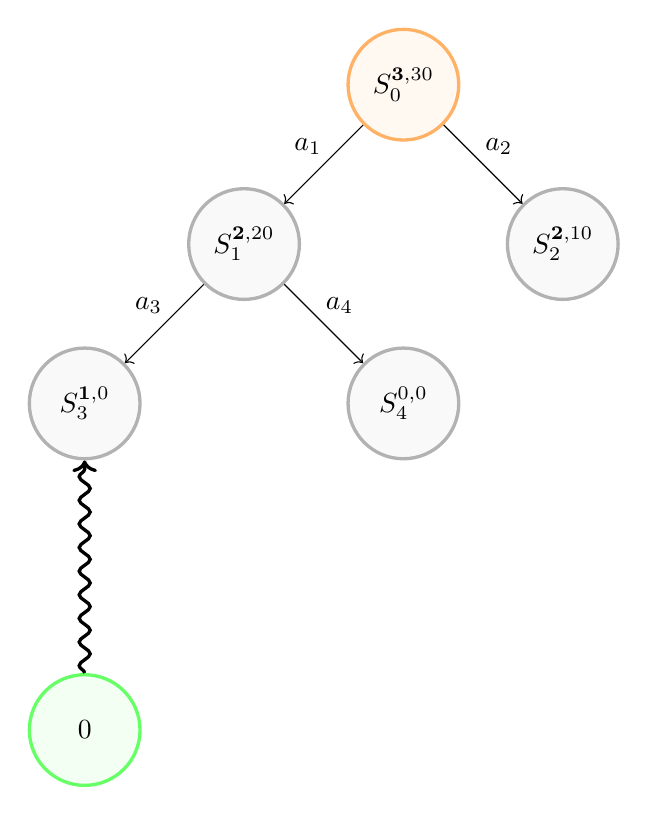
\begin{tikzpicture}[
            root_node/.style={circle, draw=orange!60, fill=orange!5, very thick, minimum size=40},
            visited_node/.style={circle, draw=green!60, fill=green!5, very thick, minimum size=40},
            unvisited_node/.style={circle, draw=gray!60, fill=gray!5, very thick, minimum size=40},
            target_node/.style={circle, draw=green!60, fill=green!5, very thick, minimum size=40},
        ]

        \node[root_node](Root){$S^{\mathbf{3},30}_0$};
        \node[unvisited_node, below left=of Root](S1){$S^{\mathbf{2},20}_1$};
        \node[unvisited_node, below right=of Root](S2){$S^{\mathbf{2},10}_2$};
        \node[unvisited_node, below left=of S1](S3){$S^{\mathbf{1},0}_3$};
        \node[unvisited_node, below right=of S1](S4){$S^{0,0}_4$};

        \node[target_node, below=of S3, yshift=-1.7cm](Target){0};

        \draw[->] (Root) -- (S1) node[midway, above, xshift=-2mm] {$a_1$};
        \draw[->] (Root) -- (S2) node[midway, above, xshift=2mm] {$a_2$};
        \draw[->] (S1) -- (S3)   node[midway, above, xshift=-2mm] {$a_3$};
        \draw[->] (S1) -- (S4)   node[midway, above, xshift=2mm] {$a_4$};
        \draw[->, very thick, decorate, decoration={snake, amplitude=.7mm, segment length=3mm}] (Target) -- (S3);
    \end{tikzpicture}
    \caption{Simulation and Backpropagation - I3}
    \label{fig:Simulation and Backpropagation - I3}
\end{figure}
\newpage
Let's do the fourth iteration $I4$ represented on Figure \ref{fig:Selection - Simulation - Backpropagation - I4}:
\begin{figure}[!ht]
    \centering
    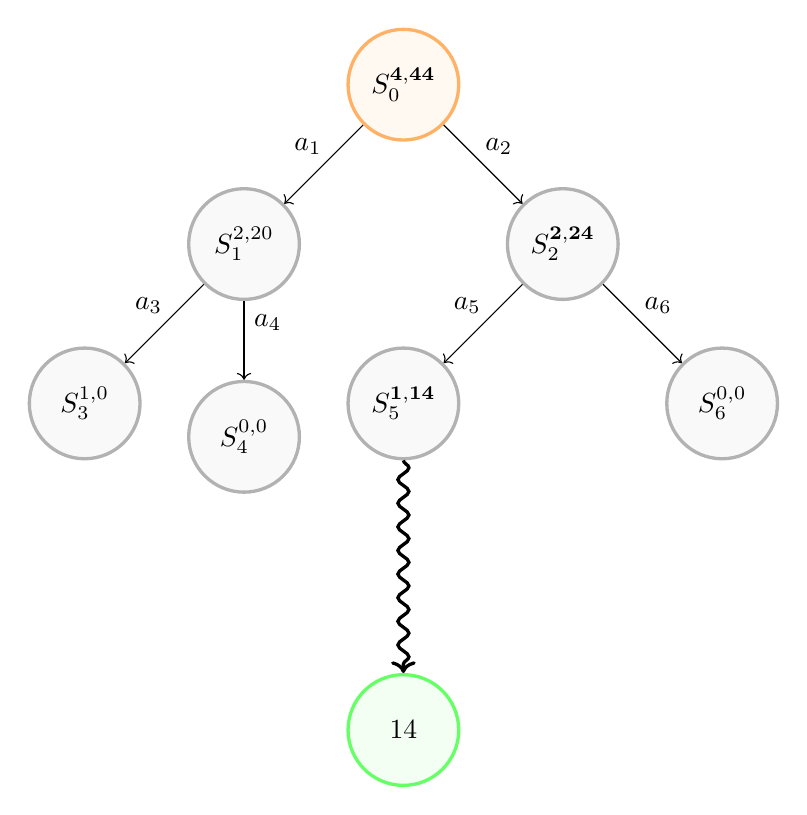
\begin{tikzpicture}[
            root_node/.style={circle, draw=orange!60, fill=orange!5, very thick, minimum size=40},
            visited_node/.style={circle, draw=green!60, fill=green!5, very thick, minimum size=40},
            unvisited_node/.style={circle, draw=gray!60, fill=gray!5, very thick, minimum size=40},
            target_node/.style={circle, draw=green!60, fill=green!5, very thick, minimum size=40},
        ]

        \node[root_node](Root){$S^{\mathbf{4,44}}_0$};
        \node[unvisited_node, below left=of Root](S1){$S^{2,20}_1$};
        \node[unvisited_node, below right=of Root](S2){$S^{\mathbf{2},\mathbf{24}}_2$};
        \node[unvisited_node, below left=of S1](S3){$S^{1,0}_3$};
        \node[unvisited_node, below=of S1](S4){$S^{0,0}_4$};
        \node[unvisited_node, below left=of S2](S5){$S^{\mathbf{1},\mathbf{14}}_5$};
        \node[unvisited_node, below right=of S2](S6){$S^{0,0}_6$};


        \node[target_node, below=of S5, yshift=-1.7cm](Target){14};

        \draw[->] (Root) -- (S1) node[midway, above, xshift=-2mm] {$a_1$};
        \draw[->] (Root) -- (S2) node[midway, above, xshift=2mm] {$a_2$};
        \draw[->] (S1) -- (S3)   node[midway, above, xshift=-2mm] {$a_3$};
        \draw[->] (S1) -- (S4)   node[midway, above, xshift=3mm] {$a_4$};
        \draw[->] (S2) -- (S5) node[midway, above, xshift=-2mm] {$a_5$};
        \draw[->] (S2) -- (S6) node[midway, above, xshift=2mm] {$a_6$};

        \draw[->, very thick, decorate, decoration={snake, amplitude=.7mm, segment length=3mm}] (S5) -- (Target);
    \end{tikzpicture}
    \caption{Selection - Simulation - Backpropagation - I4}
    \label{fig:Selection - Simulation - Backpropagation - I4}
\end{figure}

The MCTS algorithm can be either stopped because you are running out of time or because you have no more available actions. For instance, if we were to stop at this stage of the algorithm, the best action to undertake is $a_2$ because it has the higher average value: $\bar{V_1}=\frac{20}{2} \le \bar{V_2}=\frac{24}{2}$.

\subsection{The different parameters in the MCTS}


\subsection{Selection policy}
\cite{different_selection_policies}
\begin{itemize}
    \item \textbf{Upper Confidence Bound (UCB):}
          \begin{itemize}
              \item \textit{Description}: UCB is a popular selection policy in MCTS that balances exploration and exploitation using a mathematical formulation that considers both the average reward of a node and the uncertainty of that reward.
              \item \textit{Trade-offs}:
                    \begin{itemize}
                        \item \textbf{Exploration vs. Exploitation}: UCB adjusts the balance between exploring less-visited nodes and exploiting nodes with high rewards.
                        \item \textbf{Parameter Sensitivity}: The performance of UCB depends on the constant \(C_p\) in its formula, which controls the level of exploration.
                        \item \textbf{Children's Count}: UCB can lead to varying numbers of children being explored, depending on the setting of \(C_p\).
                    \end{itemize}
          \end{itemize}

    \item \textbf{UCB1-Tuned:}
          \begin{itemize}
              \item \textit{Description}: A variation of UCB that dynamically adjusts the exploration term based on the variance of rewards, making it more adaptive to different scenarios.
              \item \textit{Trade-offs}:
                    \begin{itemize}
                        \item \textbf{Adaptivity}: UCB1-Tuned can adapt to the variance in the rewards, potentially leading to better performance in complex environments.
                        \item \textbf{Computational Cost}: The added complexity in adjusting the exploration term may lead to higher computational costs.
                        \item \textbf{Children's Count}: This policy may result in fewer nodes being selected for expansion when the variance is low, focusing more on exploitation.
                    \end{itemize}
          \end{itemize}

    \item \textbf{Single-Player (SP-MCTS):}
          \begin{itemize}
              \item \textit{Description}: A variant of MCTS specifically designed for single-player scenarios, incorporating a third term in the UCB formula to account for the uncertainty in node values.
              \item \textit{Trade-offs}:
                    \begin{itemize}
                        \item \textbf{Exploration of Uncertainty}: SP-MCTS inflates the uncertainty term for less-visited nodes, which can lead to more thorough exploration in single-player settings.
                        \item \textbf{Focus on Strong Lines}: This policy tends to favor strong lines of play, potentially neglecting less promising but necessary exploratory paths.
                        \item \textbf{Children's Count}: Tends to explore a wider range of children nodes, balancing between known strong strategies and potential new solutions.
                    \end{itemize}
          \end{itemize}

    \item \textbf{Bayesian UCT:}
          \begin{itemize}
              \item \textit{Description}: Bayesian UCT integrates Bayesian statistics into the selection policy, allowing for a probabilistic approach to balancing exploration and exploitation.
              \item \textit{Trade-offs}:
                    \begin{itemize}
                        \item \textbf{Probabilistic Exploration}: Bayesian UCT provides a more nuanced exploration strategy by considering prior knowledge and updating beliefs as more information is gathered.
                        \item \textbf{Complexity}: The Bayesian approach can be computationally expensive, especially in large search spaces.
                        \item \textbf{Children's Count}: The number of children explored under Bayesian UCT can be influenced by the prior distributions used, potentially leading to more focused exploration in areas of high uncertainty.
                    \end{itemize}
          \end{itemize}
\end{itemize}

\subsection{Simulation policy}

\subsubsection{Different nodes}
\chapter{Problem Description}
\label{Chapter3}
\lhead{Chapter 3. \emph{Problem Description}}
%\todo{Present and explain your problem AHA in detail Assumptions should be stated clearly}

\section{Overview}

Kiwi's traveler wants to travel in $N$ different areas in $N$ days, let's denote $A$ the set of areas the traveler wants to visit: \[A=\{A_{1}, A_{2}, \ldots A_{{N}}\}\]
where each \(A_{j}\) is a set of airports in area \(j\):
\[
A_{j} = \{ a_{j,1}, a_{j,2}, \ldots, a_{j,k_j} \}
\]
where \( a_{j,k_j} \) being airports in area \(j\) and \(k_j\) is the number of airports in area \(j\).

The traveler has to visit one area per day. He has to leave this area to visit a new area by flying from the airport he flew in.
He leaves from a known starting airport and has to do his journey and come back to the starting area, not necessarly the starting airport. 
There are flight connections between different airports, with different prices depending on the day of the travel:
we can write $c^{d}_{ij}$ the cost to travel from $city_i$ to $city_j$ on day $d$. We do not necessarly have $c^{d}_{ij}=c^{d}_{ji}$ neither $c^{d_1}_{ij}=c^{d_2}_{ij}$ if $d_1 \neq d_2$. The problem can hence be characterised as assymetric and time dependant.

The aim of the problem is to find the cheapest route for the traveler's journey.

We can then formulate the problem more effectively:

\begin{itemize}
    \item $\mathcal{A} = \{1, 2, \ldots, N\}$: Set of areas.
    \item $A_j = \{a_{j,1}, a_{j,2}, \ldots, a_{j,k_j}\}$: Set of airports in area $j \in \mathcal{A}$.
    \item $\mathcal{D} = \{1, 2, \ldots, N\}$: Set of days.
    \item $U_d \subseteq \mathcal{A}$: Set of areas that have not been visited by the end of day $d$.
\end{itemize}

Parameters
\begin{itemize}
    \item $c_{ij}^d$: Cost to travel from airport $i$ to airport $j$ on day $d \in \mathcal{D}$.
\end{itemize}

Variables
\begin{itemize}
    \item $x_{ij}^d$: Binary variable which is 1 if the traveler flies from airport $i$ to airport $j$ on day $d$, and 0 otherwise.
    \item $v_j^d$: Binary variable which is 1 if area $j$ is visited on day $d$, and 0 otherwise.
\end{itemize}

\subsection*{Constraints}
1. Starting and Ending Constraints:
   \begin{itemize}
       \item The traveler starts at the known starting airport $S_{0}$.
       \item The traveler must return to an airport in the starting area on the final day N.
   \end{itemize}

2. Flow Constraints:
   \begin{itemize}
       \item The traveler must leave each area and arrive at the next area on consecutive days, the next area has not been visited yet.
       \item Ensure that the traveler can only fly into and out of the same airport within an area.
       \item Ensure each area is visited exactly once.
       \item Update the unvisited list as areas are visited.
   \end{itemize}

\subsection*{Objective Function}
The goal is to minimise the journey's total travel cost:
\[\min \left( \sum_{d=2}^{N-1} \sum_{i \in \bigcup\limits_{k=2}^{N-1} A_k} \sum_{j \in \bigcup\limits_{k=3}^{N} A_k} c_{ij}^d x_{ij}^d + \sum_{j \in A_1} c_{S_0,j}^1 x_{S_0,j}^1 + \sum_{i \in A_N} \sum_{j \in A_1} c_{ij}^N x_{ij}^N \right)\]

\subsection*{Constraints}
    \begin{itemize}        
        \item Starting at the known starting airport $S_{0}$ at take an existing flight connection:
        \[ \sum_{j \in A_1} x_{S_{0},j}^1 = 1 \] 
        \[ \forall d \in \mathcal{D}, c_{S_0,j}^{d} \in \mathbb{R^{+*}}\] 
        
        \item Visit exactly one airport in each area each day:
        \[ \sum_{i \in A_{d}} \sum_{j \in A_{d+1}} x_{ij}^d = 1 \quad \forall d \in \{1, 2, \ldots, N-1\} \]

        \item Ensure the traveler leaves from the same airport they arrived at the previous day:
        \[ \sum_{k \in A_d} x_{ik}^d = \sum_{k \in A_{d-1}} x_{ki}^{d-1} \quad \forall i \in \bigcup_{j=1}^N A_j, \forall d \in \{2, 3, \ldots, N\} \]

        \item Return to an airport in the starting area on the final day with an existing flight connection:
        \[ \sum_{i \in A_N} \sum_{j \in A_1} x_{ij}^N = 1 \]
        \[ \forall (i,j) \in A_N \times A_1, c_{i,j}^{N} \in \mathbb{R^{+*}}\] 

        \item Ensure each area is visited exactly once:
        \[ \sum_{d \in \mathcal{D}} v_j^d = 1 \quad \forall j \in \mathcal{A} \]

        \item Update the unvisited list:
        \[ v_j^d = 1 \implies j \notin U_d \quad \forall j \in \mathcal{A}, \forall d \in \mathcal{D} \]

        \item Ensure a flight on day $d$ between $i$ and $j$ exists only if the cost exists and $j$ is in the unvisited areas on day $d$:
        \[ x_{ij}^d \leq c_{ij}^d \cdot v_j^d \quad \forall i, j \in (\bigcup_{j=1}^N A_j)^2, \forall d \in \mathcal{D} \]
        \[ x_{ij}^d \leq v_j^d \quad \forall j \in \bigcup_{j=1}^N A_j, \forall d \in \mathcal{D} \]

        

        \item Binary variable constraints:
        \[x_{ij}^d \in \{0, 1\} \quad \forall (i, j) \in (\bigcup_{j=1}^N A_j)^2, \forall d \in \mathcal{D}\]
        \[ v_j^d \in \{0, 1\} \quad \forall j \in \mathcal{A}, \forall d \in \mathcal{D} \]

    \end{itemize}

\section{Instances}
\subsection{Description}

We are given a set of 14 Instances $I_{n}=\{I_1,I_2,...,I_{13},I_{14}\}$ that we have to solve.
Every instances has the same overall structure.

For example, the first few lines of $I_4$ are:

\begin{center}
    \begin{tabular}{l}
    \textcolor{gray}{13} \textcolor{blue}{GDN} \\
    first \\
    \textcolor{orange}{WRO} \textcolor{purple}{DL1} \\
    \textcolor{red}{second} \\
    BZG KJ1 \\
    third \\
    BXP LB1 \\
    \end{tabular}
\end{center}
    
That means that the Traveller will visit \textcolor{gray}{13} different areas, he starts from airport \textcolor{blue}{GDN}, that belongs to the starting area.
Then we are given the list of airports that are in every zone.
For example, the second zone is named \textcolor{red}{second} and has two airports: \textcolor{orange}{WRO} and \textcolor{purple}{DL1}.

After all the information regarding the areas and the airports we have the flight connections informations. In Table \ref{table:Flight connections sample I6}, few flights are displayed from $I_6$ for illustrative purpose.
\begin{table}[!ht]
    \centering
    \begin{tabular}{||cccc||} 
     \toprule
     Departure from & Arrival & Day & Cost \\ [1ex] 
     \midrule
     KKE & BIL & 1  & 19  \\ 
     UAX & NKE & 73 & 16  \\
     UXA & BCT & 0  & 141 \\
     UXA & DBD & 0  & 112 \\
     UXA & DBD & 0  & 128 \\
     UXA & DBD & 0  & 110 \\
     [1ex] 
     \bottomrule
    \end{tabular}
    \caption{Flight connections sample I6}
    \label{table:Flight connections sample I6}
\end{table}


For every instance $I_i$, we know what connections exist between two airports for a specific day and the associated cost.
There might be in some instances flights connections at day 0, this means these connections exist for every day of the journey at the same price.
\\Furthermore, we could have same flight connections at a specific day but with different prices. We then have to consider only the more relevant connections i.e.\ the flight connection with the lowest fare.

\subsection{General formulation}

An instance \(I_i\) can be mathematically defined as follows:

\[
I_i = (N_i, S_{i0}, A_{i}, F_{i})
\]

where:

\begin{itemize}
    \item \textbf{Number of Areas} \(N_i\):
    \[
    N_i \in \mathbb{N}
    \]
    The total number of distinct areas in instance \(I_i\).
    
    \item \textbf{Starting Airport} \(S_{i0}\):
    \[
    S_{i0} \in \text{Airports}
    \]
    The starting airport of the traveller.
    
    \item \textbf{Airports in Each Area}:
    \[A_{i}=
    \{A_{i,1}, A_{i,2}, \ldots A_{i,{N_i}}\}
    \]
    where each \(A_{i,j}\) is a set of airports in area \(j\) for instance \(i\):
    \[
    A_{i,j} = \{ a_{i,j,1}, a_{i,j,2}, \ldots, a_{i,j,k_j} \}
    \]
    with \( a_{i,j,k_j} \) being airports in area \(j\) and \(k_j\) is the number of airports in area \(j\).
    
    \item \textbf{Flight Connections}:
    \[F_{i}=
    \{F_{i,0},F_{i,1}, F_{i,2}, \ldots, F_{i,N_i}\}
    \]
    where each flight matrix \( F_{i,k} \) represents the flight information of instance $i$ on day \(k\):
    \[
    F_{i,k} = \begin{pmatrix}
    a_{i,k,1}^d & a_{i,k,1}^a & f_{i,k,1} \\
    a_{i,k,2}^d & a_{i,k,2}^a & f_{i,k,2} \\
    \vdots & \vdots & \vdots \\
    a_{i,k,l_{k,i}}^d & a_{i,k,l_{k,i}}^a & f_{i,k,l_{k,i}}
    \end{pmatrix}
    \]

    \begin{itemize}
        \item \textbf{Columns}:
        \begin{itemize}
            \item Departure Airport: \( a_{i,k,j}^d \) (Departure airport for the \(j\)-th flight on day \(k\))
            \item Arrival Airport: \( a_{i,k,j}^a \) (Arrival airport for the \(j\)-th flight on day \(k\))
            \item Cost: \( f_{i,k,j} \) (Cost of the \(j\)-th flight on day \(k\)), where \( j \in [1, l_{k,i}] \)
            \end{itemize}
        \item \textbf{Rows}: 
        Each row corresponds to a specific flight on day \(k\). The number of rows \(l_{k,i}\) depends on the number of flights available on that day.
    \end{itemize}

\end{itemize}


\subsection{Kiwi's rules}
When solving all the instances, Kiwi's defined time limits constraints based on the nature of the instance. We can summarise these constraints in the Table above:
\begin{table}[!ht]
    \centering
    \begin{tabular}{||cccc||} 
     \toprule
     Instance & nb areas & Nb Airports & Time limit (s) \\ [1ex] 
     \midrule
     Small  & $\leq 20$  & $<50$  & 3  \\ 
     Medium & $\leq 100$ & $<200$ & 5  \\
     Large  & $>100$     &        & 15 \\ [1ex] 
     \bottomrule
    \end{tabular}
    \caption{Time limits based on the number of areas and airports}
    \label{table:Time limit constraints}
\end{table}

All the useful information about the instances such as the starting airport, the associated area, the range of airports per area, the number of airports and the time limit constraints defined in  Table \ref{table:Time limit constraints}.

\begin{table}[!ht]
    \centering
    \resizebox{\textwidth}{!}{ % Resize the table to fit the text width
    \begin{tabular}{||>{\centering\arraybackslash}p{2.2cm} 
                        >{\centering\arraybackslash}p{4cm} 
                        >{\centering\arraybackslash}p{1.8cm} 
                        >{\centering\arraybackslash}p{3.2cm} 
                        >{\centering\arraybackslash}p{2.2cm} 
                        >{\centering\arraybackslash}p{2.2cm} ||} 
     \toprule
     Instances & \makecell{Starting \\ Area - Airport} & \makecell{N° \\ areas} & \makecell{Min - Max \\ airport per area} & \makecell{N° \\ Airports} & \makecell{Time \\ Limit (s)} \\ [1ex] 
     \midrule
     I1  & Zona\_0 - AB0 & 10  & 1 - 1 & 10   &  3  \\  
     I2  & Area\_0 - EBJ & 10  & 1 - 2 & 15   &  3  \\  
     I3  & ninth - GDN & 13  & 1 - 6 & 38   &  3  \\  
     I4  & Poland - GDN & 40  & 1 - 5 & 99   &  5  \\  
     I5  & zone0 - RCF & 46  & 3 - 3 & 138  &  5  \\ 
     I6  & zone0 - VHK & 96  & 2 - 2 & 192  &  5  \\ 
     I7  & abfuidmorz - AHG & 150 & 1 - 6 & 300  &  15 \\ 
     I8  & atrdruwkbz - AEW & 200 & 1 - 4 & 300  &  15 \\ 
     I9  & fcjsqtmccq - GVT & 250 & 1 - 1 & 250  &  15 \\ 
     I10 & eqlfrvhlwu - ECB & 300 & 1 - 1 & 300  &  15 \\ 
     I11 & pbggaefrjv - LIJ & 150 & 1 - 4 & 200  &  15 \\ 
     I12 & unnwaxhnoq - PJE & 200 & 1 - 4 & 250  &  15 \\ 
     I13 & hpvkogdfpf - GKU & 250 & 1 - 3 & 275  &  15 \\ 
     I14 & jjewssxvsc - IXG & 300 & 1 - 1 & 300  &  15 \\ [1ex] 
     \bottomrule
    \end{tabular}
    }
    \caption{Instances and their respective parameters}
    \label{table:Instances presentation}
\end{table}

\newpage


\chapter{Methodology}
\label{Chapter4}
\lhead{Chapter 4. \emph{Methodology}}
\todo{Describe implementation details}
\newpage

\tikzset{class/.style={rectangle, draw=green!60, fill=green!5, very thick, minimum size=20},
    method/.style={rectangle, draw=yellow!60, fill=yellow!5, very thick, minimum size=20},
    attributes/.style={rectangle, draw=blue!60, fill=blue!5, very thick, minimum size=20},
    instance/.style={rectangle, draw=orange!60, fill=orange!5, very thick, minimum size=20}
}


\section{Monte Carlo Tree Search implementation}
\subsection{General flow}

Based on the discussion in Chapter \ref{Chapter2}, the flow of the Monte Carlo Tree Search algorithm is summarised in Figure \ref{fig:Flow MCTS}:
\begin{figure}[!ht]
    \centering
    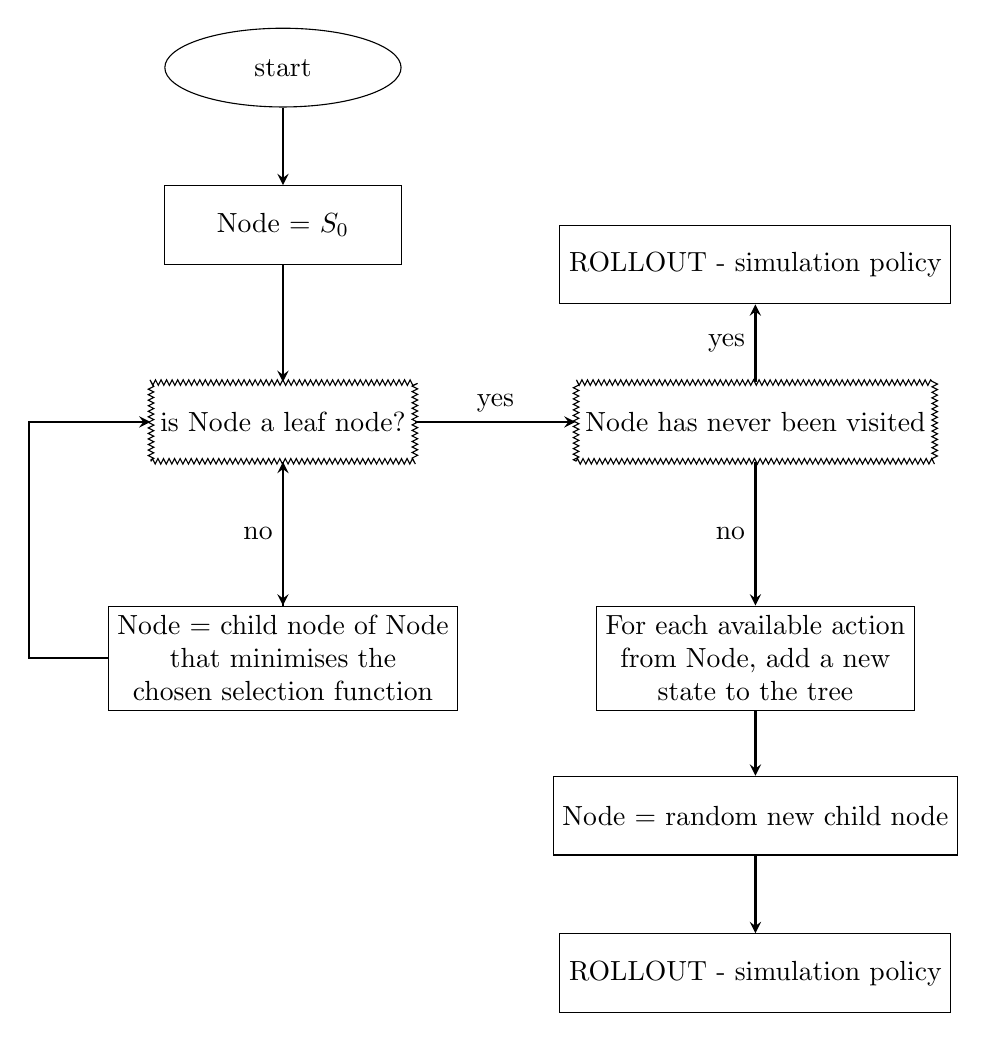
\begin{tikzpicture}[
            startstop/.style={ellipse, minimum width=3cm, minimum height=1cm, text centered, draw=black},
            process/.style={rectangle, minimum width=3cm, minimum height=1cm, text centered, draw=black},
            decision/.style={rectangle, minimum width=3cm, minimum height=1cm, text centered, draw=black, decorate, decoration={zigzag,segment length=2,amplitude=1}},
            arrow/.style={thick,->,>=stealth},
            node distance=2cm
        ]

        \node (start) [startstop] {start};
        \node (current) [process, below of=start] {Node = $S_0$};
        \node (decision1) [decision, below of=current, yshift=-0.5cm] {is Node a leaf node?};
        \node (ucb1) [process, below of=decision1, yshift=-1cm, align=center] {Node = child node of Node \\ that minimises the \\ chosen selection function};
        \node (decision2) [decision, right of=decision1, xshift=4cm] {Node has never been visited};
        \node (expand) [process, below of=decision2, yshift=-1cm, align=center] {For each available action\\ from Node, add a new \\ state to the tree};
        \node (firstChild) [process, below of=expand] {Node = random new child node};
        \node (rollout1) [process, below of=firstChild] {ROLLOUT - simulation policy};
        \node (rollout2) [process, above of=decision2] {ROLLOUT - simulation policy};

        \draw [arrow] (start) -- (current);
        \draw [arrow] (current) -- (decision1);
        \draw [arrow] (decision1) -- node[anchor=east] {no} (ucb1);
        \draw [arrow] (ucb1) -- (decision1);
        \draw [arrow] (decision1) -- node[anchor=south] {yes} (decision2);
        \draw [arrow] (decision2) -- node[anchor=east] {no} (expand);
        \draw [arrow] (decision2) -- node[anchor=east] {yes} (rollout2);
        \draw [arrow] (expand) -- (firstChild);
        \draw [arrow] (ucb1.west) -- ++(-1,0) |- (decision1.west);
        \draw [arrow] (firstChild) -- (rollout1);

    \end{tikzpicture}
    \caption{Flow MCTS}
    \label{fig:Flow MCTS}
\end{figure}

For every iteration of this algorithm - there are four different phases:

\begin{enumerate}
    \item \textbf{Selection:} Starting from the root node (the starting airport $S_{i0}$ for $I_{i}$), select successive child nodes (airports that are in unvisited areas) until a leaf node (the airport in the initial area - not necessarly the starting airport) is reached. Use the chosen Selection function to evaluate which node's is the most promising. In the illustrative example in Section \ref{subsub:Example}, we used the UCB1 function for the selection function. We were also dealing with a maximisation problem, hence we selected nodes with the highest UCB1 value. A contrario, in Kiwi's minimisation problem,  nodes are evaluated based on the lowest value of the selection function.

    \item \textbf{Expansion:} If the selected node is not a terminal node, expand the tree by adding all possible child nodes.

    \item \textbf{Simulation:} From the newly added node, perform a simulation (based on the simulation policy) until we reach a terminal node i.e\ we find a feasible solution.

    \item \textbf{Backpropagation:} Update the values of the nodes along the path from the newly added node to the root based on the result of the simulation.

          \begin{equation}
              \mathcal{B}(S^{n_i,t_i}_i) = S^{n_i+1,t_i+\mathcal{R}(S^{n_i,t_i}_i)}_i
          \end{equation}

          where $\mathcal{R}(S^{n_i,t_i}_i)$ is the cost of the solution found after performing a simulation from node $S^{n_i,t_i}_i$.
\end{enumerate}


\newpage
\subsubsection{Data Preprocessing}

In order to implement our MCTS' solution, the first thing to implement was a data\_preprocessing \tikz[baseline=(class.base)]{\node[class] (class) {class};} in order to preprocess the given instance.
Kiwi's challenge has been solved using Python 3.10 on VS Code 1.92.2. Our Python code is structured using object-oriented programming. This data\_preprocessing class is represented on Figure \ref{fig:data_preprocessing_class}.
The input is an \tikz[baseline=(instance.base)]{\node[instance] (instance) {instance};} $I_i$, as defined in Chapter \ref{Chapter3}:

\begin{figure}[!ht]
    \centering
    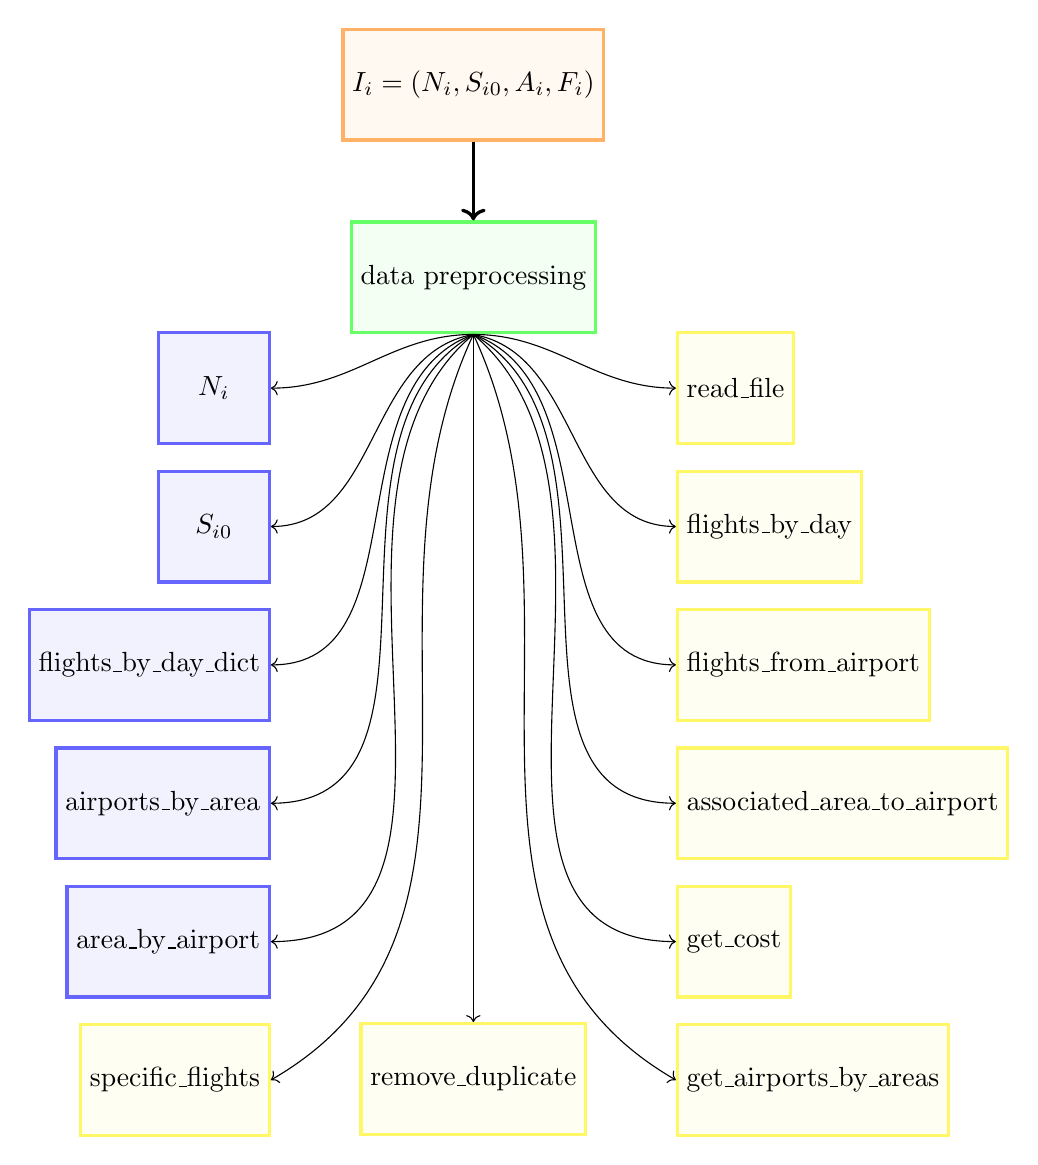
\begin{tikzpicture}[
            class/.style={rectangle, draw=green!60, fill=green!5, very thick, minimum size=40},
            methods/.style={rectangle, draw=yellow!60, fill=yellow!5, very thick, minimum size=40},
            attributes/.style={rectangle, draw=blue!60, fill=blue!5, very thick, minimum size=40},
            instance/.style={rectangle, draw=orange!60, fill=orange!5, very thick, minimum size=40}
        ]

        %Nodes  
        \node[instance]          (Instance){$I_i = (N_i, S_{i0}, A_{i}, F_{i})$};
        \node[class]             (Class)[below=of Instance]{data preprocessing};

        \node[attributes, left=of  Class , yshift=-40] (Attr1) {$N_i$};
        \node[attributes, left=of  Class , yshift=-90] (Attr2) {$S_{i0}$};
        \node[attributes, left=of  Class , yshift=-140] (Attr3) {flights\_by\_day\_dict};
        \node[attributes, left=of  Class, yshift=-190] (Attr4) {airports\_by\_area};
        \node[attributes, left=of  Class, yshift=-240] (Attr5) {area\_by\_airport};
        %\node[methods, left=of Class, yshift=-290, align=center] (Meth10) {flights\_from\_airport\_at\_a\_\\specific\_day\_with\_previous\_areas};
        \node[methods, left=of Class, yshift=-290, align=center] (Meth10) {specific\_flights};


        \node[methods, right=of  Class, yshift=-40] (Meth1) {read\_file};
        \node[methods, right=of  Class, yshift=-90] (Meth2) {flights\_by\_day};
        \node[methods, right=of  Class, yshift=-140] (Meth3) {flights\_from\_airport};
        \node[methods, right=of  Class, yshift=-190] (Meth4) {associated\_area\_to\_airport};
        \node[methods, right=of  Class, yshift=-240] (Meth5) {get\_cost};
        \node[methods, right=of  Class, yshift=-290] (Meth6) {get\_airports\_by\_areas};
        \node[methods, below=of  Class, yshift=-220] (Meth7) {remove\_duplicate};

        %Lines
        \draw[->, very thick] (Instance.south)  to node[midway, right] {} (Class.north);

        \draw[->] (Class.south) to[out=180, in=0] (Attr1.east);
        \draw[->] (Class.south) to[out=190, in=0] (Attr2.east);
        \draw[->] (Class.south) to[out=200, in=0] (Attr3.east);
        \draw[->] (Class.south) to[out=210, in=0] (Attr4.east);
        \draw[->] (Class.south) to[out=220, in=0] (Attr5.east);

        % Arrows from Class to Methods (right side)
        \draw[->] (Class.south) to[out=0, in=180] (Meth1.west);
        \draw[->] (Class.south) to[out=350, in=180] (Meth2.west);
        \draw[->] (Class.south) to[out=340, in=180] (Meth3.west);
        \draw[->] (Class.south) to[out=330, in=180] (Meth4.west);
        \draw[->] (Class.south) to[out=320, in=180] (Meth5.west);

        \draw[->] (Class.south) to[out=-115, in=30] (Meth10.east);
        \draw[->] (Class.south) to[out=-65, in=150] (Meth6.west);
        \draw[->] (Class.south) to[out=-90, in=90] (Meth7.north);
    \end{tikzpicture}
    \caption{Explanation of the data preprocessing class}
    \label{fig:data_preprocessing_class}
\end{figure}

Different useful \tikz[baseline=(methods.base)]{\node[method] (methods) {methods};} are implemented within the data\_preprocessing class to compute and manage various attributes required for the problem at hand. These methods are designed to prepare and structure the data, making it easier to use in subsequent phases of the algorithm.
For example, the remove\_duplicate method ensures that only the cheapest flight connections are considered between two airports if multiple flight connections exist at different prices on the same day.
Other methods, such as flights\_by\_day\_dict and get\_airports\_by\_areas organise the data. The first method regroup all the flights by their respective days, creating a dictionary where each key represents a day and its corresponding value is a list of available flights. The second is regrouping all the airports present in the different areas.
Finally, others methods like specific\_flights will be helpful in the algorithm's development gives all the possible flight connections from a specific airport on a specific day considering the visited\_areas, it hence gives you all the possibles actions from a node.

Given that Python is relatively slower in terms of computation compared to other programming languages, we opted to use as much as possible dictionaries. Dictionnaries allow for efficient data retrieval based on a key, with an average time complexity of $\mathcal{O}(1)$. This choice enhances the performance of the data preprocessing step, ensuring that the algorithm runs more efficiently despite Python’s inherent limitations.

\newpage
\subsubsection{Node}
\label{subsub:node}
\begin{figure}[h]
    \centering
    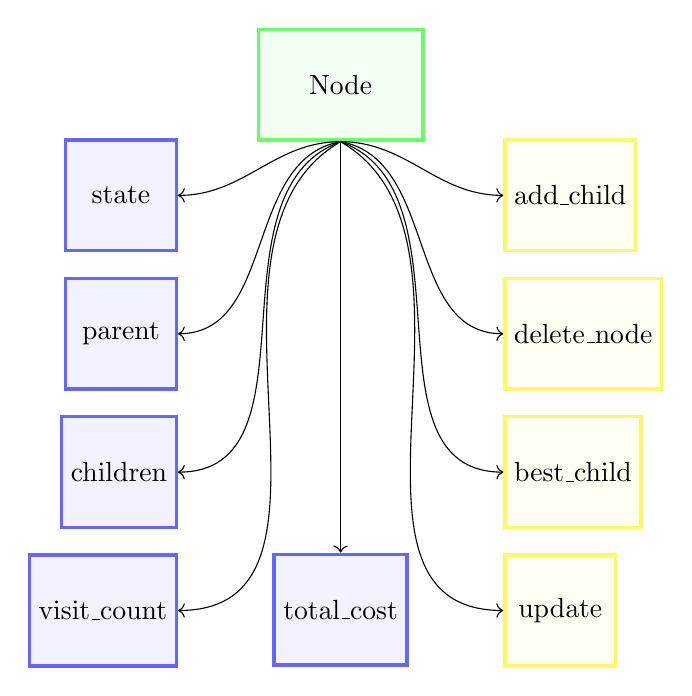
\begin{tikzpicture}[
            class/.style={rectangle, draw=green!60, fill=green!5, very thick, minimum size=40},
            methods/.style={rectangle, draw=yellow!60, fill=yellow!5, very thick, minimum size=40},
            attributes/.style={rectangle, draw=blue!60, fill=blue!5, very thick, minimum size=40},
            instance/.style={rectangle, draw=orange!60, fill=orange!5, very thick, minimum size=40}
        ]

        \node[class]             (Class){\phantom{-----}Node\phantom{-----}};

        \node[attributes, left=of  Class , yshift=-40] (Attr1) {state};
        \node[attributes, left=of  Class , yshift=-90] (Attr2) {parent};
        \node[attributes, left=of  Class , yshift=-140] (Attr3) {children};
        \node[attributes, left=of  Class, yshift=-190] (Attr4) {visit\_count};

        \node[methods, right=of  Class, yshift=-40] (Meth1) {add\_child};
        \node[methods, right=of  Class, yshift=-90] (Meth2) {delete\_node};
        \node[methods, right=of  Class, yshift=-140] (Meth3) {best\_child};
        \node[methods, right=of  Class, yshift=-190] (Meth4) {update};

        \node[attributes, below=of  Class, yshift=-120] (Meth5) {total\_cost};


        \draw[->] (Class.south) to[out=180, in=0] (Attr1.east);
        \draw[->] (Class.south) to[out=190, in=0] (Attr2.east);
        \draw[->] (Class.south) to[out=200, in=0] (Attr3.east);
        \draw[->] (Class.south) to[out=210, in=0] (Attr4.east);

        \draw[->] (Class.south) to[out=0, in=180] (Meth1.west);
        \draw[->] (Class.south) to[out=350, in=180] (Meth2.west);
        \draw[->] (Class.south) to[out=340, in=180] (Meth3.west);
        \draw[->] (Class.south) to[out=330, in=180] (Meth4.west);

        \draw[->] (Class.south) to[out=-90, in=90] (Meth5.north);

    \end{tikzpicture}
    \caption{Explanation of the Node class}
    \label{fig:node_class}
\end{figure}

As mentionned earlier in Section \ref{subsub:Example}, we use a Node structure in our algorithm, hence we implemented a Node class.
Each Node has a reference to a parent node (unless it is the root node) and may have one or more child nodes (unless it is a leaf node). These relationships form a tree structure where each node can expand into potential future states, guiding the search process.
The visit\_count tracks the number of times a node has been visited during the MCTS process. This is crucial for evaluating the node’s importance and for calculating score of the node with the selection function.
The state is a dictionnary that contains node's current information:
\begin{itemize}
    \item current\_airport: The airport where the traveler is  at this node.
    \item current\_day: The day of the trip at this node.
    \item remaining\_zones: The zones that still need to be visited to complete the journey.
    \item visited\_zones: The zones that have already been visited to ensure that all zones are visited exactly once during the trip.
    \item total\_cost: It represents the accumulated cost of the current solution path leading to this node.
\end{itemize}

Additionally, to manage the expansion of child nodes, the add\_child method is defined.
This method generates new nodes based on the possible actions available from the current node, the potential flight connections from the current airport on this specific day, given the current path taken so far. These new nodes represent the next possible states in the traveler’s journey, allowing the search tree to expand and explore different travel routes.
Finally, the delete\_node method can be used to delete a node from the list of its parent's children.


\section{The different policies}
In the previous section, we outlined the general flow of the MCTS algorithm, focusing on two cores classes, data\_preprocessing and Node, that are central in MCTS' implementation.

In Section \ref{sub:selection_policies_litterature}, we explored the various selection policies that guide the decision-making process within MCTS.
Although there is a limited litterature review, we decided to parameterise not only the selection policy but also the simulation and expansion policy.

\subsection{Simulation policies}
When you simulate from a given node in the tree, the goal is to find a feasible combinaison of airport that could be a solution to our problem.
Then from this current node, you have the current state (defined in Section \ref{subsub:node}), so you have to chose for the remaining actions based on the simulation policy.

We decided to define three distinct simulation policies:

\begin{itemize}
    \item Random policy: This policy selects a random action from the set of available actions, introducing variability and exploration in the simulation process.
    \item Greedy Policy: This policy selects the action that corresponds to the cheapest available flight connection, thus prioritising cost minimisation at each step.

    \item Tolerance Policy (with coefficient $c$):
          This policy selects an action randomly from a subset of actions that are within a certain tolerance level of the minimum cost action. The tolerance level is defined by a coefficient $c$, allowing for a balance between exploration and exploitation.

          The tolerance heuristic is defined as follows:
          \begin{itemize}
              \item Identify the cheapest flight connection among the available actions $c_{min}$.
              \item Filter the actions to include only those with a cost less or equal than $c_{min}(1+c) $.
              \item Randomly select an action from this filtered set.
          \end{itemize}

\end{itemize}

\subsection{Expansion policies}
When expanding a node, it’s theoretically possible to expand all available child nodes i.e.\ add all the possible flight connections from a node at a specific day to the tree. However, in practice, this can be computationally expensive and time-consuming, particularly in problems with a large number of possible actions. To address this, heuristic approaches often involve compromises that enhance the efficiency of the search process by selectively expanding certain nodes rather than all possible ones.

In our implementation we defined two expansion policies:

\begin{itemize}
    \item \textbf{Top-K Actions Policy}: This policy expands the nodes corresponding to the cheapest flight connections available. Specifically, it sorts all possible actions based on their associated costs and selects the top \(k\) actions with the lowest costs, where \(k\) is regulated by a parameter called \texttt{number\_of\_children}. This approach ensures that only the most promising actions, in terms of cost efficiency, are considered during expansion. This policy narrow down the search space but can reach to local optima.
    \item \textbf{Ratio Best-Random Policy}: This policy takes a more balanced approach by combining the selection of the best actions with a degree of randomness. First, it calculates the number of top actions to select based on a predefined ratio, \(c\), of \texttt{number\_of\_children}. The top actions are chosen based on their costs, similar to the Top-K Actions Policy. After selecting these best actions, the policy randomly selects additional actions from the remaining pool to reach the desired number of children. This policy is designed to explore a broader range of possibilities while still prioritising cost-effective options.
\end{itemize}

In addition to these policies, as already mention, the parameter \texttt{number\_of\_children} plays a critical role in regulating the maximum number of children that can be expanded from any given node. This limitation controls the size of the search tree, especially in larger instances where again, expanding too many nodes could make the algorithm computationally exhaustive.

\subsection{MCTS' Pseudo-code}
In this section, we go into more detail about how we implemented the algorithm in practice by examining the different functions of our MCTS class. The main idea is:

\begin{algorithm}[H]
    \caption{Monte\_Carlo\_Tree\_Search}
    \label{alg:MCTS}
    \begin{algorithmic}[1]
        \STATE Initialise Root\_Node with Initial\_State
        \WHILE{Tree is not fully explored}
        \STATE $Node \leftarrow \text{Select}(Root\_Node)$
        \IF{$Node$ is not fully expanded}
        \STATE $Node \leftarrow \text{Expand}(Node)$
        \ENDIF
        \STATE $Cost \leftarrow \text{Simulate}(Node)$
        \STATE \text{Backpropagate}($Node$, $Cost$)
        \ENDWHILE
        \RETURN $Best\_Leaf\_Node$
    \end{algorithmic}
\end{algorithm}

The \texttt{Select} function returns two arguments: a boolean and a node. The boolean indicates to the expansion function whether expansion is necessary (True means no expansion needed, False means yes):

\begin{algorithm}[H]
    \caption{Select\_Function}
    \label{alg:SelectFunction}
    \begin{algorithmic}[1]
        \STATE \textbf{Input:} $Node$
        \STATE $Current \leftarrow Node$
        \WHILE{$Current.Children$ is not empty}
        \IF{Current is not fully expanded}
        \STATE $UnvisitedChildren \leftarrow \text{Children with } VisitCount = 0$
        \IF{$UnvisitedChildren$ is not empty}
        \STATE $SelectedChild \leftarrow \text{Randomly select from } UnvisitedChildren$
        \RETURN $True, SelectedChild$
        \ENDIF
        \ELSE
        \STATE $Current \leftarrow \text{BestChild}(Current)$
        \ENDIF
        \ENDWHILE
        \IF{$Current.Children$ is empty \textbf{and} $Current.State["current\_day"]==N_{Areas}$}
        \RETURN $False, Current$
        \ELSIF{$Current.Children$ is empty \textbf{and} $Current.State["current\_day"]==N_{Areas}$}
        \RETURN $False, Current$
        \ELSIF{$Current.State["current\_day"]==N_{Areas} + 1$}
        \RETURN $True, Current$
        \ENDIF
    \end{algorithmic}
\end{algorithm}

We backpropagate the node using the update method of the node. The new node becomes the parent of this node, and we do that until \texttt{Node} is \texttt{None}, i.e., we have backpropagated all the information up to the root node.

\begin{algorithm}[H]
    \caption{Backpropagate\_Function}
    \label{alg:Backpropagate}
    \begin{algorithmic}[1]
        \WHILE{$Node$ is not $None$}
        \STATE $Node.Update(Cost)$
        \STATE $Node \leftarrow Node.Parent$
        \ENDWHILE
    \end{algorithmic}
\end{algorithm}

The transition function modifies the states of a node by updating the current airport, the visited zones, remaining zones, etc.

\begin{algorithm}[H]
    \caption{Transition\_Function}
    \label{alg:TransitionFunction}
    \begin{algorithmic}[1]
        \STATE $New\_State \leftarrow \text{Copy of } State$
        \STATE $New\_State.Current\_Day \leftarrow State.Current\_Day + 1$
        \STATE $New\_State.Current\_Airport \leftarrow Action[0]$
        \STATE $New\_State.Total\_Cost \leftarrow State.Total\_Cost + Action[1]$
        \STATE \text{Update}($New\_State.Path$, $New\_State.Current\_Airport$)
        \STATE \text{Remove\_Visited}($New\_State.Remaining\_Zones$, $New\_State.Current\_Airport$)
        \STATE \text{Add\_Visited}($New\_State.Visited\_Zones$, $New\_State.Current\_Airport$)
        \RETURN $New\_State$
    \end{algorithmic}
\end{algorithm}

Finally, the Best Child function, defined in the Node class is based on the selection function UCB, UCB1\_Tuned, SP and Bayesian, computes the score of the visited nodes and pick the one that minimises the selection function.

\begin{algorithm}[H]
    \caption{Best Child}
    \label{alg:Best Child}
    \begin{algorithmic}[1]
        \REQUIRE $Selection\_Function$
        \STATE $Visited\_Children \leftarrow \text{Children with } visitCount > 0$
        \STATE $Choices\_Weights \leftarrow \left[ Selection\_Function(child) \text{ for child in } Visited\_Children \right]$
        \STATE $Best\_Child\_Node \leftarrow \text{Child with minimum } Choices\_Weights$
        \RETURN $Best\_Child\_Node$
    \end{algorithmic}
\end{algorithm}
\chapter{Results and performance}
\label{Chapter5}
\lhead{Chapter 5. \emph{Results and performance}}

\todo{Present the results and discuss any differences between the findings and your initial predictions/hypothesis}

\todo{Interpret your experimental results - do not just present lots of data and expect the reader to understand it.
    Evaluate what you have achieved against the aims and objectives you outlined in the introduction}

\section{Hypothesis}
As mentionned in Section \ref{section:research_obj}, the primary objective was to implement a new algorithm in order to find solutions without imposing time constraints. Only instances ($I_1 \ldots I_8$) are studied because they represent realistic scenarios.

Hence, simulations for every instances have been conducted, testing different combinations of parameters in what is called a grid search. Each combination of parameters was run 10 times to ensure the reliability and consistency of the results.
One challenge, is that the computational budget is limited when using Python. Especially for the more complex instance, ($I_7 \ldots I_{14}$) where the time to find a solution for a given set of parameters is more than 20 minutes. It becomes practically impossible to perform for each instance, 10 simulations for every combination of parameters in the grid search. Hence, the size of the grid search for the more complex instances were reduced as shown in Table \ref{table:Grid search}.

\begin{table}[!ht]
    \centering
    \caption{Grid search}
    \resizebox{\textwidth}{!}{ % Resize the table to fit the text width
        \begin{tabular}{||>{\centering\arraybackslash}p{3cm}
            >{\centering\arraybackslash}p{4.5cm}
            >{\centering\arraybackslash}p{3.5cm}
            >{\centering\arraybackslash}p{2cm}||}
            \toprule
                                          & ($I_1 \ldots I_6$)        & ($I_7 \ldots I_8$) & ($I_9 \ldots I_{14}$) \\ [1ex]
            \midrule
            \textit{selection\_policies}  & top\_k, ratio\_k          & top\_k, ratio\_k   & -                     \\
            \textit{simulation\_policies} & random, greedy, tolerance & greedy             & -                     \\
            \textit{selection\_policies}  & UCB, UCB1T                & UCB, UCB1T         & -                     \\
            \textit{c\_p}                 & 0, 1.4, 2.8               & 1.4                & -                     \\
            \textit{N\_children}          & 5, 10, 15                 & 10                 & -                     \\
            \textit{Ratio}                & 0, .3, .5, .8, 1          & .5                 & -                     \\
            \bottomrule
        \end{tabular}
    }
    \label{table:Grid search}
\end{table}

\section{Results analysis}
\subsection{Overview}

After running the various simulations with the search grid parameters defined in Table \ref{table:Grid search}, our results were compared with those of Kiwi and RL (Reinforcement Learning) \cite{reinforcement_learning_yaro} - the only two official publications on this challenge.

\begin{table}[!ht]
    \centering
    \caption{Best results vs State of the art}
    \resizebox{.8\textwidth}{!}{ % Resize the table to fit the text width
        \begin{tabular}{||>{\centering\arraybackslash}p{1.5cm}
            >{\centering\arraybackslash}p{1.5cm}
            >{\centering\arraybackslash}p{1.5cm}
            >{\centering\arraybackslash}p{1.5cm}
            >{\centering\arraybackslash}p{1.5cm}
            >{\centering\arraybackslash}p{1.5cm}
            >{\centering\arraybackslash}p{1.5cm} ||}
            \toprule
            Instance & Kiwi's & RL     & Best known & Best found    & Mean    & Std   \\ [1ex]
            \midrule
            I1       & 1396   & 1396   & 1396       & \textbf{1396} & 1396    & 0     \\
            I2       & 1498   & 1498   & 1498       & \textbf{1498} &         &       \\
            I3       & 7672   & 7672   & 7672       & \textbf{7672} &         &       \\
            I4       & 14024  & 13952  & 13952      & 15101         & 16208.8 & 520.8 \\
            I5       & 698    & 690    & 690        & -             & -       & -     \\
            I6       & 2159   & 2610   & 2159       & -             & -       & -     \\
            I7       & 31681  & 30937  & 30937      & -             &         &       \\
            I8       & 4052   & 4081   & 4052       & \textbf{4037} & -       &       \\
            I9       & 76372  & 75604  & 75604      & -             & -       & -     \\
            I10      & 21667  & 58304  & 21667      & -             & -       & -     \\
            I11      & 44153  & 59361  & 44153      & -             & -       & -     \\
            I12      & 65447  & 86074  & 65447      & -             & -       & -     \\
            I13      & 97859  & 166543 & 97859      & -             & -       & -     \\
            I14      & 118811 & 198787 & 118811     & -             & -       & -     \\ [1ex]
            \bottomrule
        \end{tabular}
    }
    \label{table:Best result vs state of the art}
\end{table}

A solution was found for $I_1, \ldots, I_4$ and $I_7, I_8$. The results shown in table \ref{table:Best result vs state of the art} are the best found costs' solution within the grid search. The results of the simulations for $I_1,\ldots I_4$ are displayed in Section \ref{AppendixC} and the detailed path-solution for these instances can be found in Section \ref{AppendixD}.
\newpage
\subsection{Analysis}
\subsubsection{I1, I2 and I3}
For these three instances, the best known solutions were found and the various simulations were carried out successfully. Therefore, the influence of the parameters on the final solution was investigated. For $I_3$, the analysis focuses on the $C_p$ parameter, the influence of the expansion ratio and finally the study will investigate the overall correlation matrix.

\subsubsection*{Analysis on $C_p$}
\begin{figure}[!ht]
    \centering
    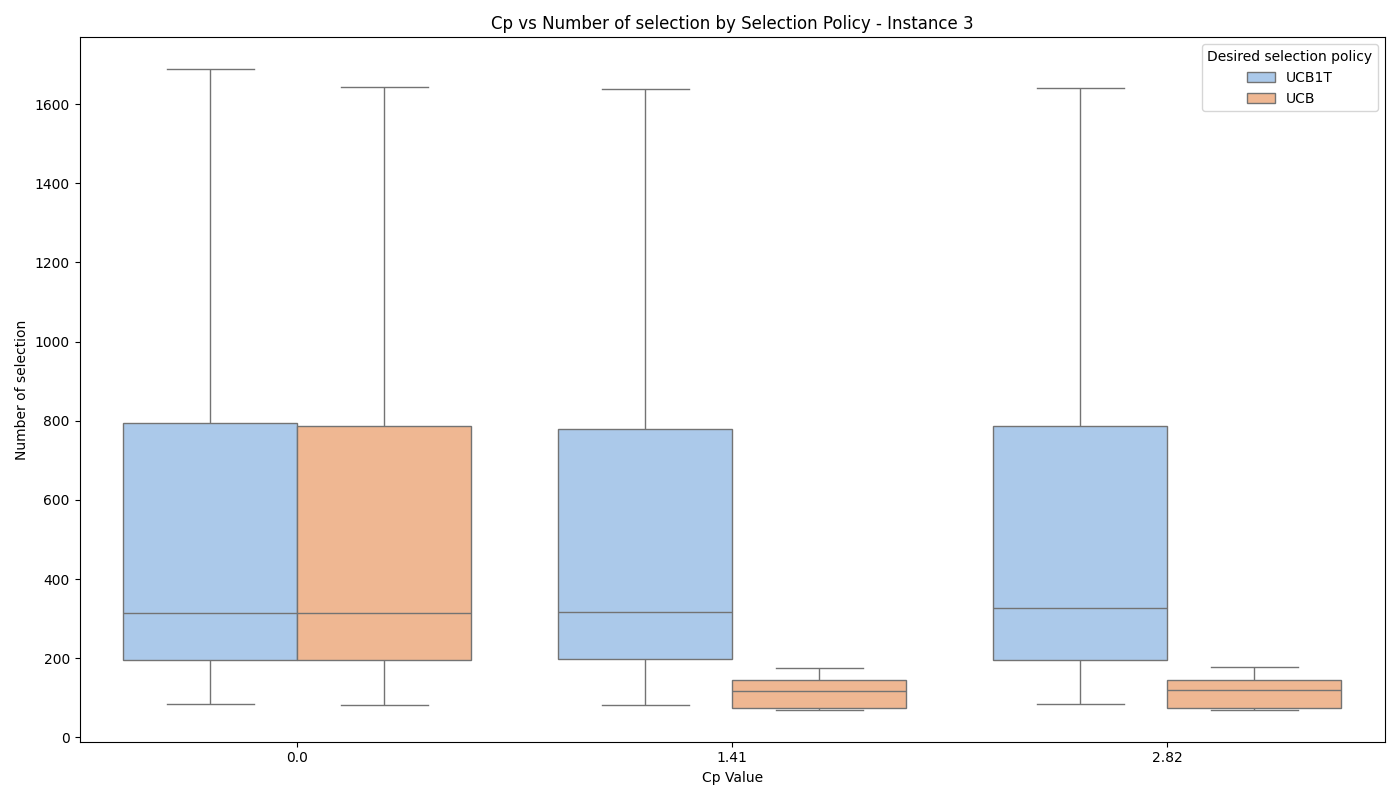
\includegraphics[width=\textwidth]{Figures/3 - cp_vs_selection.png}
    \caption{$C_p$ vs Number of selection}
    \label{fig:cp_vs_selection_3}
\end{figure}

On Figure \ref{fig:cp_vs_cost_3} the box plots illustrate the relationship between the exploration constant \( C_p \) and the number of selection phases under the UCB and UCB1T selection policies:

\begin{itemize}
    \item \textbf{\( C_p = 0 \) lead to the same performance:}
          When the $C_p=0$, the selection policy of the UCB and the UCB1T are the same (cf equation \ref{eq:UCB} and \ref{eq:UCB1T}).
    \item \textbf{Higher \( C_p \) values lead to faster convergence for UCB:}
          As \( C_p \) increases from $0.0$ to $2.82$, the median number of selection phases under UCB policy decreases. A higher number of selection for the UCB policy could be expected, as $C_p$ increases but for small instances it convergences faster.

    \item \textbf{UCB1T Encourages More Exploration:}
          UCB1T consistently results in a higher number of selection phases compared to UCB, especially at higher \( C_p \) values. This is consistent with UCB1T's definition to promote broader exploration before converging.

    \item \textbf{Balance Between Exploration and Exploitation:}
          The choice of \( C_p \) should be based on the specific problem, balancing the need for exploration (higher \( C_p \)) with the desire for quicker convergence (lower \( C_p \)).
\end{itemize}

Although a higher exploration parameter $C_p$ may lead to faster convergence under the UCB selection policy, it often results in worse outcomes compared to the UCB1T algorithm, as shown on Figure \ref{fig:cp_vs_cost_3}.
\begin{figure}[!ht]
    \centering
    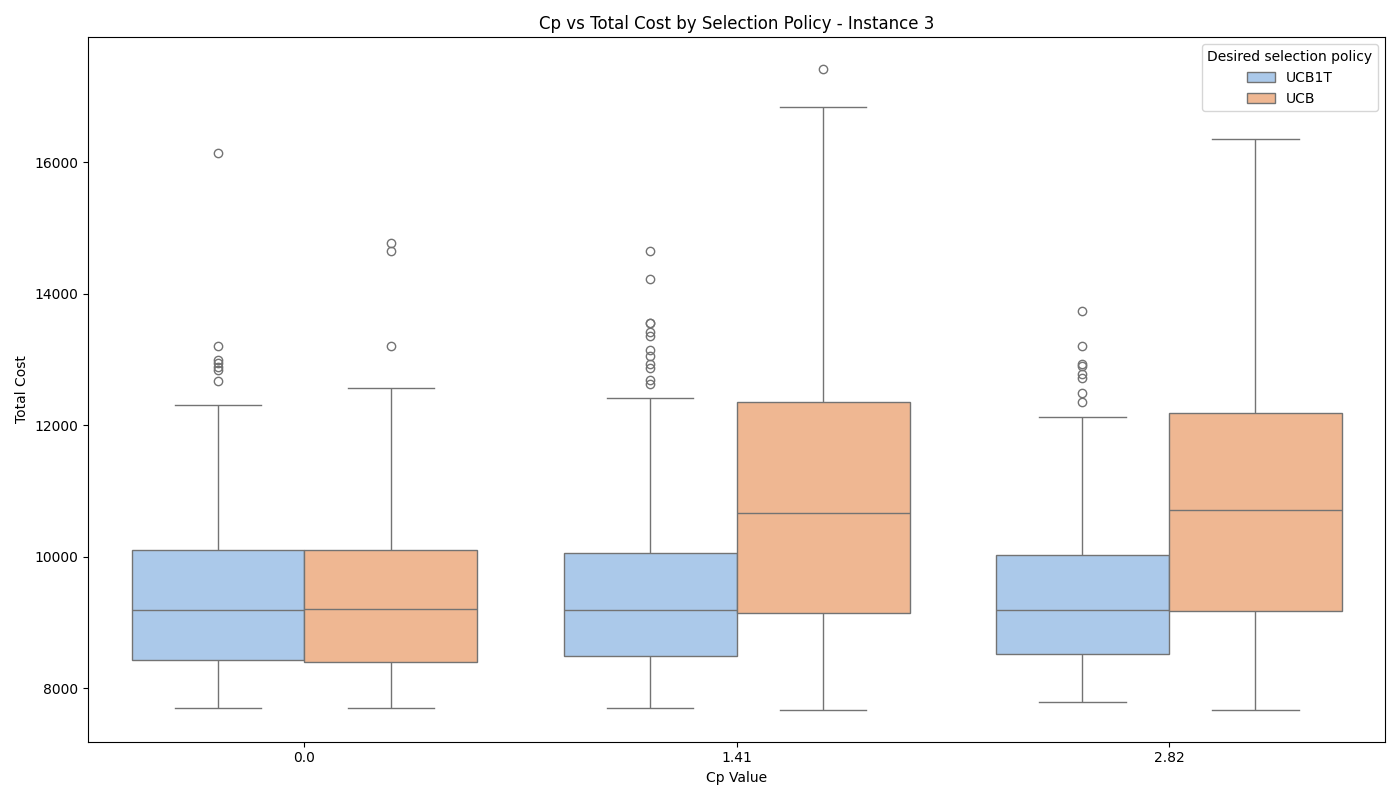
\includegraphics[width=\textwidth]{Figures/3 - cp_vs_cost.png}
    \caption{$C_p$ vs Total cost}
    \label{fig:cp_vs_cost_3}
\end{figure}
While UCB1T may require more time to converge, it generally explores the search tree more effectively, leading to better overall performance.





\subsubsection*{Analysis of Expansion ratio}

\begin{figure}[!ht]
    \centering
    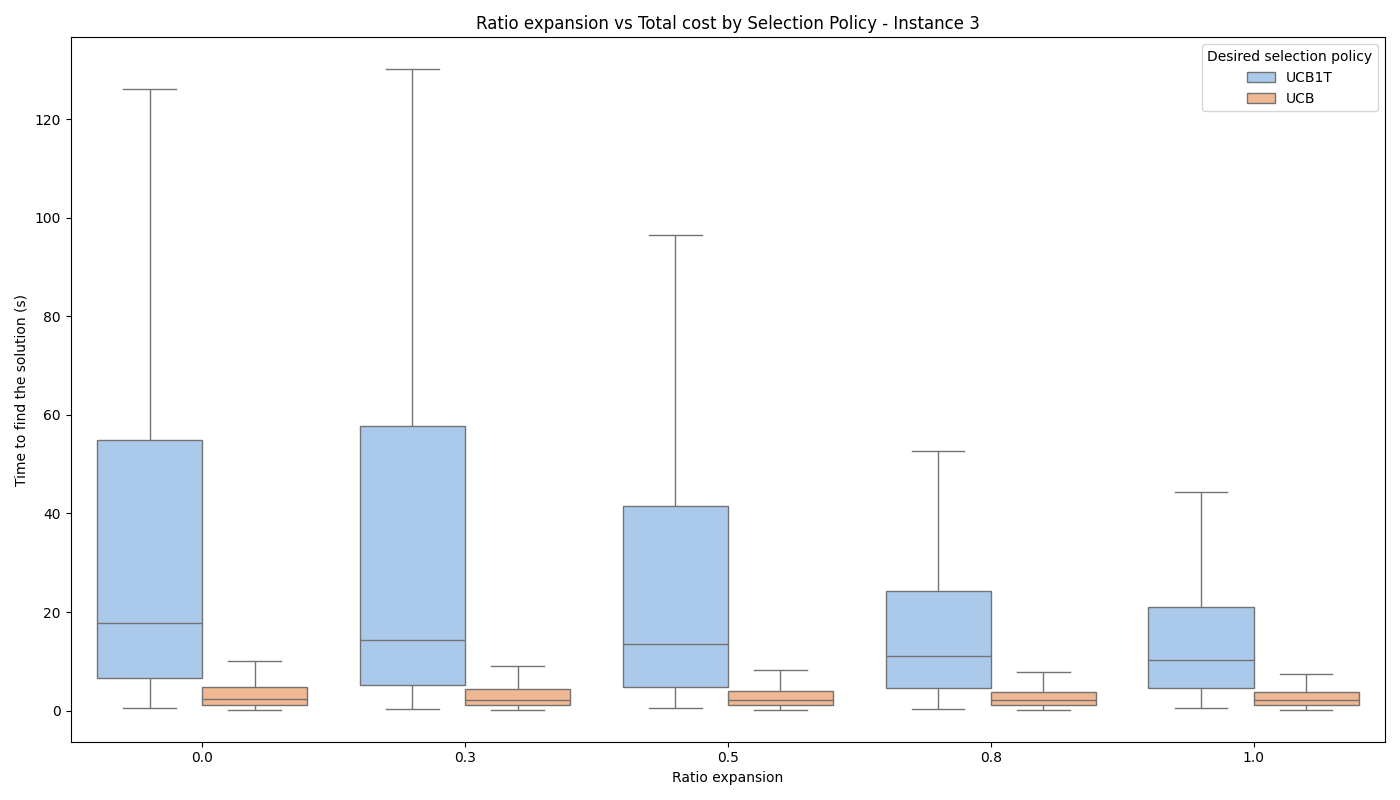
\includegraphics[width=\textwidth]{Figures/3 - ratio_vs_time.png}
    \caption{Ratio expansion vs Time to find the solution}
    \label{fig:Ratio vs Time}
\end{figure}

The box plots show the relationship between ratio expansion (the proportion of expanded child nodes that has the cheapest flight connection over the chosen number of children) and the time to find a solution for the UCB and UCB1T policies:

\begin{itemize}
    \item \textbf{UCB is More Time-Efficient:}
          Across all ratio expansion values, the UCB policy consistently finds solutions more quickly than UCB1T. This suggests that UCB, being less aggressive in exploration, converges on solutions faster.

          %\item \textbf{UCB1T Takes Longer Due to Extensive Exploration:}
          %      UCB1T shows higher and more variable times to find solutions, especially at lower ratio expansions (e.g., $0.0$). This reflects UCB1T's property to explore more than UCB.

    \item \textbf{Higher Ratio Expansions Lead to Quicker Solutions:}
          For both policies, the time to find a solution generally decreases as the ratio expansion increases, indicating a more efficient search process when more expanded nodes lead to solutions. However, in more complex instances, it is crucial to have a ratio $r \in [0.3,0.7]$ to escape potential leaf node.
\end{itemize}

Finally, the UCB policy is more correlated to the expansion ratio than the UCB1T as shown on Figure \ref{fig:ratio_vs_cost_3}.
\begin{figure}[!ht]
    \centering
    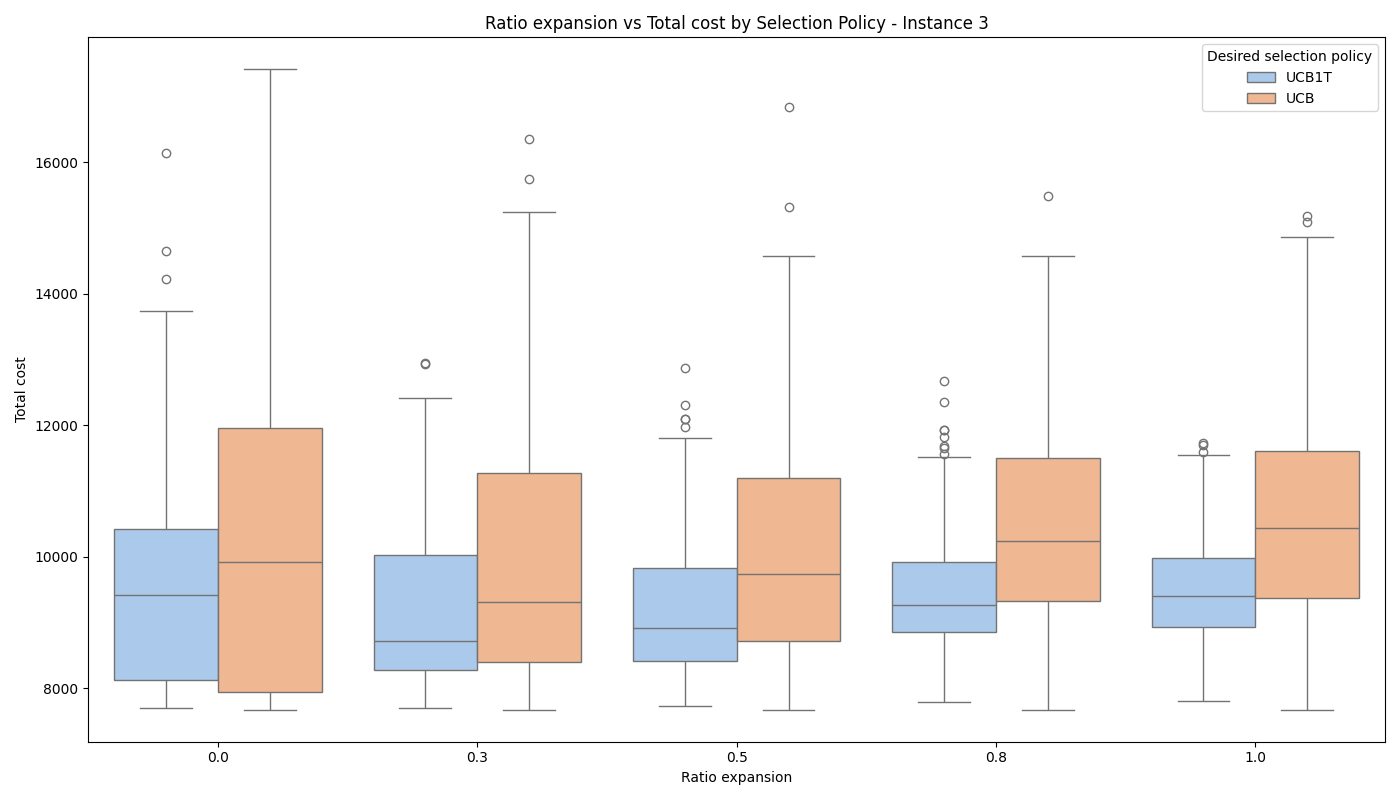
\includegraphics[width=\textwidth]{Figures/3 - ratio_vs_cost.png}
    \caption{Expansion ratio vs Total cost}
    \label{fig:ratio_vs_cost_3}
\end{figure}

UCB's overall performance is worst than UCB1T because it relies heavily on the exploitation compared to UCB1T that even if it converges slower gives better result.


\subsubsection{I5 and I6}

The challenge faced with these two instances is that the defined selection, simulation and expansion policy were not robust enough to explore the tree effectively.

After all the simulations, some nodes in the tree—under the random policy, were able to simulate until reaching a final state. However, due to the randomness of the policy, the tree was pruned at each further iteration where a solution could not be found.

\subsubsection{I4, I7 and I8}

For these instances we have found
\chapter{Conclusion}
\label{Chapter6}
\lhead{Chapter 6. \emph{Conclusion}}

\todo{Explain what conclusions you have come to as a result of doing this work. Lessons learnt and what would you do different next time. Please summarise the key recommendations at the end of this section, in no more than 5 bullet points.}

\section{Summary of Work}
\label{section:Summary}

\section{Critics}
\label{section:Critics}

\section{Future Work}
\label{section:finalDiscussion}


\todo{The References section should include a full list of references. Avoid having a list of web sites. Examiners may mark you down very heavily if your references are mainly web sites.}







\chapter{Progress and next steps}
\label{Chapter7}
\lhead{Chapter 7. \emph{Progress and next steps}}


%-----------------
%	APPENDICES
%-----------------
%\addtocontents{toc}{\vspace{2em}} % Add a gap in the Contents, for aesthetics
%\appendix
\chapter{Code Listings}
\label{AppendixA}
\lhead{Appendix A. \emph{Code Listings}}

\section{Data preprocessing}
\begin{lstlisting}[language = Python]
    import numpy as np
    from copy import deepcopy
    
    
    class data_preprocessing:
        def __init__(self, instance_path):
            self.instance_path = instance_path
    
            self.info, self.flights = self.read_file(f_name=self.instance_path)
            self.number_of_areas, self.starting_airport = (
                int(self.info[0][0]),
                self.info[0][1],
            )
    
            self.flights_by_day_dict = self.flights_by_day(flight_list=self.flights)
    
            self.flights_by_day_dict = self.remove_duplicate(
                flights_by_day=self.flights_by_day_dict
            )
    
            self.list_days = [k for k in range(1, self.number_of_areas)]
    
            self.airports_by_area = self.get_airports_by_areas()
            self.area_to_explore = self.which_area_to_explore(
                airports_by_area=self.airports_by_area
            )
            self.area_by_airport = self.invert_dict(original_dict=self.airports_by_area)
    
            self.starting_area = self.associated_area_to_airport(
                airport=self.starting_airport
            )
            self.list_airports = self.get_list_of_airports()
            self.list_areas = list(self.airports_by_area.keys())
            self.areas_connections_by_day = (
                self.possible_flights_from_zone_to_zone_specific_day()
            )
    
        def read_file(self, f_name):
            dist = []
            line_nu = -1
            with open(f_name) as infile:
                for line in infile:
                    line_nu += 1
                    if line_nu == 0:
                        index = int(line.split()[0]) * 2 + 1
                    if line_nu >= index:
                        temp = line.split()
                        temp[2] = int(temp[2])
                        temp[3] = int(temp[3])
                        dist.append(temp)
                    else:
                        dist.append(line.split())
                info = dist[: int(dist[0][0]) * 2 + 1]
                flights = dist[int(dist[0][0]) * 2 + 1 :]
            return info, flights
    
        def flights_by_day(self, flight_list):
            # Create an empty dictionary to hold flights organized by day
            flights_by_day = {}
    
            # Iterate over each flight in the input list
            for flight in flight_list:
                # Extract the day from the flight entry
                day = flight[2]
    
                # Create a flight entry without the day
                flight_without_day = flight[:2] + flight[3:]
    
                # Add the flight to the corresponding day in the dictionary
                if day not in flights_by_day:
                    flights_by_day[day] = []
                flights_by_day[day].append(flight_without_day)
    
            return flights_by_day
    
        def flights_from_airport(self, flights_by_day, from_airport, considered_day):
            flights_from_airport = []
            for day, flights in flights_by_day.items():
                if day == considered_day:
                    for flight in flights:
                        if flight[0] == from_airport:
                            flights_from_airport.append(flight)
                    return flights_from_airport
                else:
                    return None
    
        def invert_dict(self, original_dict):
            inverted_dict = {}
            for key, value_list in original_dict.items():
                for value in value_list:
                    if value in inverted_dict:
                        inverted_dict[value].append(key)
                    else:
                        inverted_dict[value] = key
            return inverted_dict
    
        def get_cost(self, day, from_airport, to_airport):
            # Retrieve flights for the specified day and day 0
            flights_day = self.flights_by_day_dict.get(day, [])
            flights_day_0 = self.flights_by_day_dict.get(0, [])
    
            # Find the cost for the specified day
            cost_day = next(
                (
                    flight[2]
                    for flight in flights_day
                    if flight[0] == from_airport and flight[1] == to_airport
                ),
                float("inf"),
            )
    
            # Find the cost for day 0
            cost_day_0 = next(
                (
                    flight[2]
                    for flight in flights_day_0
                    if flight[0] == from_airport and flight[1] == to_airport
                ),
                float("inf"),
            )
    
            # Return the minimum cost if either exists, otherwise inf
            if cost_day == float("inf") and cost_day_0 == float("inf"):
                return float("inf")
    
            return min(cost_day, cost_day_0)
    
        def possible_flights_from_zone_to_zone_specific_day(self):
            areas_connections_by_day = {}
    
            for day, flights in self.flights_by_day_dict.items():
                areas_connections_list = []
    
                for flight in flights:
                    connection = f"{self.area_by_airport.get(flight[0])} to {self.area_by_airport.get(flight[1])}"
                    if connection not in areas_connections_list:
                        areas_connections_list.append(connection)
    
                areas_connections_by_day[day] = areas_connections_list
    
            return areas_connections_by_day
    
        def get_airports_by_areas(self):
            area_num = int(self.info[0][0])
            return {f"{i}": self.info[2 + i * 2] for i in range(0, area_num)}
    
        def get_list_of_airports(self):
            unique_airports = set()
    
            # Iterate through each sublist and add elements to the set
            for sublist in self.airports_by_area.values():
                for airport in sublist:
                    unique_airports.add(airport)
    
            return list(unique_airports)
    
        def associated_area_to_airport(self, airport):
            return next(
                (
                    area
                    for area, airports in self.airports_by_area.items()
                    if airport in airports
                ),
                "Airport not found",
            )
    
        def remove_duplicate(self, flights_by_day):
            for day, flights in flights_by_day.items():
                unique_flights = {}
                for flight in flights:
                    flight_key = (flight[0], flight[1])
                    if flight_key not in unique_flights:
                        unique_flights[flight_key] = flight
                    else:
                        if flight[2] < unique_flights[flight_key][2]:
                            # print(flight[0],flight[1],flight[2],flight_key,unique_flights[flight_key][2])
                            unique_flights[flight_key] = flight
                    flights_by_day[day] = list(unique_flights.values())
            return flights_by_day
    
        def possible_flights_from_an_airport_at_a_specific_day(self, day, from_airport):
            daily_flights = self.flights_by_day_dict.get(day, [])
    
            flights_from_airport = []
            for flight in daily_flights:
                if flight[0] == from_airport:
    
                    flights_from_airport.append([flight[1], flight[2]])
    
            return flights_from_airport
    
        def possible_flights_from_an_airport_at_a_specific_day_with_previous_areas(
            self, day, from_airport, visited_areas
        ):
            daily_flights = self.flights_by_day_dict.get(
                day, []
            ) + self.flights_by_day_dict.get(0, [])
            flights_from_airport = []
            for flight in daily_flights:
                # print(self.associated_area_to_airport(airport=flight[0]))
                if (flight[0] == from_airport) and (
                    self.associated_area_to_airport(airport=flight[1]) not in visited_areas
                ):
    
                    flights_from_airport.append([flight[1], flight[2]])
    
            return flights_from_airport
    
        def which_area_to_explore(self, airports_by_area):
            return list(
                {
                    key: len(value)
                    for key, value in airports_by_area.items()
                    if len(value) > 1
                }
            )
    

\end{lstlisting}
\newpage
\section{Node}
\begin{lstlisting}[language = Python]
    

import numpy as np
import random
from scipy.stats import (
kstest,
norm,
beta,
expon,
gamma,
lognorm,
weibull_min,
uniform,
pareto,
t,
chi2,
)


class Node:
def __init__(self, state, desired_selection_policy, cp, parent=None):
self.cp = cp
self.desired_selection_policy = desired_selection_policy
self.state = state  # State is a dictionary representing the current situation
self.parent = parent  # Parent node
self.children = []  # List of child nodes
self.visit_count = 0  # Number of times this node has been visited
self.total_cost = 0  # Total cost accumulated in simulations from this node
self.scores = []

def add_child(self, child_state):
child_node = Node(
state=child_state,
desired_selection_policy=self.desired_selection_policy,
cp=self.cp,
parent=self,
)
self.children.append(child_node)
return child_node

def is_fully_expanded(self):
# if self.parent is None:
#    return False
return len(self.children) > 0 and all(
child.visit_count > 0 for child in self.children
)

def update(self, result):
self.visit_count += 1
self.total_cost += result
self.scores.append(result)

def UCB(self, c_param):
epsilon = 0

visited_children = [child for child in self.children if (child.visit_count > 0)]

sorted_children = sorted(
visited_children,
key=lambda child: child.total_cost / (child.visit_count + epsilon),
)
scores = {child: rank + 1 for rank, child in enumerate(sorted_children)}
total_scores = sum(scores.values())

def normalized_score(child):
return scores[child] / total_scores

choices_weights = [
normalized_score(child)
+ c_param
* (2 * np.log(self.visit_count) / (child.visit_count + epsilon)) ** 0.5
for child in visited_children
]

best_child_node = self.children[np.argmin(choices_weights)]

return best_child_node

def SP(self):
visited_children = [child for child in self.children if child.visit_count > 0]
D = 1

def sp_mcts_score(child):
mean_cost = np.mean(child.scores) if len(child.scores) > 0 else 0
variance = np.var(child.scores) if len(child.scores) > 0 else 0
possible_deviation = np.sqrt(variance + (D / child.visit_count))
return mean_cost - self.cp * possible_deviation

choices_weights = [sp_mcts_score(child) for child in visited_children]

best_child_node = self.children[np.argmin(choices_weights)]
return best_child_node

def Bayesian(self):
visited_children = [child for child in self.children if child.visit_count > 0]
N = self.visit_count

def bayesian_uct_score(child, use_variance=False):
mean_cost = np.mean(child.scores) if len(child.scores) > 0 else 0
exploration_term = np.sqrt(2 * np.log(N) / child.visit_count)

if use_variance:
variance = np.sqrt(np.var(child.scores)) if len(child.scores) > 0 else 0
exploration_term *= variance

return mean_cost + exploration_term

# Select which Bayesian UCT formula to use
use_variance = True  # Change this to `False` to use the first formula
choices_weights = [
bayesian_uct_score(child, use_variance=use_variance)
for child in visited_children
]

best_child_node = self.children[np.argmin(choices_weights)]
return best_child_node

def UCB1_tuned(self, c_param):
visited_children = [child for child in self.children if child.visit_count > 0]

def ucb1_tuned_score(child):
mean_cost = np.mean(child.scores) if len(self.scores) > 1 else 0
variance = np.var(self.scores) if len(self.scores) > 1 else 0
# UCB1-Tuned formula
exploration_term = np.sqrt(
(np.log(self.visit_count) / child.visit_count)
* min(
0.25,
variance
+ np.sqrt(2 * np.log(self.visit_count) / child.visit_count),
)
)
return mean_cost + c_param * exploration_term

choices_weights = [ucb1_tuned_score(child) for child in visited_children]

best_child_node = self.children[np.argmin(choices_weights)]
return best_child_node

def thompson_sampling(self, c_param):
visited_children = [child for child in self.children if child.visit_count > 0]

def best_fit_distribution(scores):
distributions = {
"normal": norm,
"beta": beta,
"exponential": expon,
"gamma": gamma,
"lognormal": lognorm,
"weibull_min": weibull_min,
"uniform": uniform,
"pareto": pareto,
"t": t,
"chi2": chi2,
}
p_values = {}
for dist_name, dist in distributions.items():
try:
params = dist.fit(scores)
d_statistic, p_value = kstest(scores, dist_name, args=params)
p_values[dist_name] = p_value
except Exception as e:
p_values[dist_name] = (
0  # Handle the error and skip this distribution
)
print(f"Skipping {dist_name} due to fitting issues: {e}")

best_dist_name = max(p_values, key=p_values.get)
best_p_value = p_values[best_dist_name]

if best_p_value < 0.05:
return None, None

best_dist = distributions[best_dist_name]
best_params = best_dist.fit(scores)

return best_dist, best_params

sampled_values = []
for child in visited_children:
if len(child.scores) > 1:
best_dist, best_params = best_fit_distribution(child.scores)
if best_dist is not None:
sampled_value = best_dist.rvs(*best_params)
sampled_values.append(sampled_value)
else:
return self.UCB(
c_param
)  # Fallback to UCB if no good distribution is found
else:
sampled_values.append(np.mean(child.scores))

best_child_node = visited_children[np.argmin(sampled_values)]
return best_child_node

def randomized_ucb(self, c_param, random_factor=0.1):
visited_children = [child for child in self.children if child.visit_count > 0]

def randomized_ucb_score(child):
mean_cost = np.mean(child.scores) if len(child.scores) > 0 else 0
exploration_term = np.sqrt(
(2 * np.log(self.visit_count) / (child.visit_count))
)
random_term = random_factor * np.random.rand()
return mean_cost + c_param * exploration_term + random_term

choices_weights = [randomized_ucb_score(child) for child in visited_children]

best_child_node = visited_children[np.argmin(choices_weights)]
return best_child_node

def epsilon_greedy(self, epsilon):
visited_children = [child for child in self.children if child.visit_count > 0]

if np.random.rand() < epsilon:
# Explore: randomly select a child
best_child_node = np.random.choice(visited_children)
else:
# Exploit: select the child with the best average cost
best_child_node = min(
visited_children,
key=lambda child: (
np.mean(child.scores) if len(child.scores) > 0 else float("inf")
),
)

return best_child_node

def best_child(self):
if self.desired_selection_policy == "UCB":
return self.UCB(c_param=self.cp)
if self.desired_selection_policy == "UCB1T":
return self.UCB1_tuned(c_param=self.cp)
if self.desired_selection_policy == "SP":
return self.epsilon_greedy(self.cp)
if self.desired_selection_policy == "Bayesian":
return self.Bayesian()

else:
raise ValueError(
f"Unknown Selection policy: {self.desired_selection_policy}"
)

def delete_node(self):
self.parent.children = [
child for child in self.parent.children if child != self
]
\end{lstlisting}
\newpage
\section{MCTS}

\begin{lstlisting}[language = Python]
    import numpy as np
import random
from copy import deepcopy
import logging
import time
import os
import shutil
import glob

from Data_Preprocessing import data_preprocessing
from Node import Node


class MCTS(data_preprocessing):
    def __init__(
        self,
        instance,
        instance_number,
        number_childrens,
        desired_expansion_policy,
        ratio_expansion,
        desired_simulation_policy,
        desired_selection_policy,
        cp,
        number_simulation,
    ):
        self.instance_number = instance_number
        self.number_childrens = number_childrens
        self.desired_simulation_policy = desired_simulation_policy
        self.desired_expansion_policy = desired_expansion_policy
        self.ratio_expansion = ratio_expansion
        self.number_simulation = number_simulation
        self.desired_selection_policy = desired_selection_policy
        self.cp = cp

        self.expanded_nodes = []
        self.simulations_dict = {}

        self.start_time = time.time()
        super().__init__(instance_path=instance)
        self.end_time_data_preprocessing = time.time() - self.start_time
        self.simulation()
        # self.organise_log_files_in_folder(
        #    folder_path=os.path.dirname(self.instance_path)
        # )
        # self.collect_all_nodes()

    def configure_logging(self):
        log_file = f"{self.instance_path}_{self.number_childrens}_{self.desired_simulation_policy}_{self.desired_expansion_policy}_{self.ratio_expansion}_{self.number_simulation}_{self.desired_selection_policy}_{self.cp}.log"
        log_file = self.get_unique_log_file(log_file)

        # Clear any existing handlers
        for handler in logging.root.handlers[:]:
            logging.root.removeHandler(handler)

        # Configure the logger
        logging.basicConfig(
            level=logging.DEBUG,  # Set the log level to DEBUG to capture all types of logs
            format="%(asctime)s - %(name)s - %(levelname)s - %(message)s",
            handlers=[
                logging.FileHandler(
                    log_file, mode="w"
                ),  # 'w' to overwrite the log file each run, 'a' to append
                # logging.StreamHandler(),  # Optional: to also print logs to the console
            ],
        )
        logger = logging.getLogger(__name__)
        return logger

    def get_unique_log_file(self, base_log_file):
        """
        Check if the log file exists and if so, create a new file with a unique suffix.
        """
        base_name, extension = os.path.splitext(base_log_file)
        counter = 0  # Start with 0 to have the first file as _0
        while True:
            new_log_file = f"{base_name}_{counter}{extension}"
            if not os.path.exists(new_log_file):
                return new_log_file
            counter += 1

    def organise_log_files_in_folder(self, folder_path):
        """
        Organize log files in the specified folder by moving files with the same base name into a dedicated directory.

        :param folder_path: Path to the folder containing the log files.
        """
        # Change to the target directory
        os.chdir(folder_path)

        # Find all log files in the directory
        log_files = glob.glob("*.log")

        # Track which files have already been moved to avoid duplication
        processed_bases = set()

        for log_file in log_files:
            # Extract the base name (up to the first '_')
            base_name = (
                log_file.rsplit("_", 1)[0]
                if "_" in log_file
                else log_file.rsplit(".", 1)[0]
            )

            if base_name not in processed_bases:
                # Mark this base as processed
                processed_bases.add(base_name)

                # Create a pattern to match all similar files
                pattern = f"{base_name}*.log"

                # Find all files matching this pattern
                matching_files = glob.glob(pattern)

                if matching_files:
                    # Create a directory for these files
                    folder_name = os.path.join(folder_path, base_name)
                    os.makedirs(folder_name, exist_ok=True)

                    # Move each matching file into the directory
                    for file in matching_files:
                        shutil.move(file, folder_name)

                    # print(
                    #    f"Moved files with base '{base_name}' into folder: {folder_name}"
                    # )

    def initialise_root_node(self):
        return {
            "current_day": 1,
            "current_airport": self.starting_airport,
            "remaining_zones": [
                x for x in self.list_areas if x != self.starting_area
            ],  # Exclude the starting area
            "visited_zones": [self.starting_area],  # Exclude the starting area
            "total_cost": 0,
            "path": [self.starting_airport],
        }

    def transition_function(self, state, action):
        new_state = deepcopy(state)
        new_state["current_day"] += 1
        new_state["current_airport"] = action[0]
        new_state["total_cost"] += action[1]
        new_state["path"].append(action[0])
        # self.logger.info(
        #    f"Airport {action[0]}, {self.associated_area_to_airport(airport=action[0])} to remove in {new_state['remaining_zones']}"
        # )
        new_state["remaining_zones"].remove(
            self.associated_area_to_airport(airport=action[0])
        )
        new_state["visited_zones"].append(
            self.associated_area_to_airport(airport=action[0])
        )
        return new_state

    def random_policy(self, actions):

        if not actions:
            return None
        return random.choice(actions)

    def greedy_policy(self, actions):

        # self.logger.info(f"Actions: {actions}")
        if not actions:
            return None
        # Select the action with the lowest cost
        best_action = min(actions, key=lambda x: x[1])
        # self.logger.info(f"Chosen action based on heuristic policy: {best_action}")
        return best_action

    def tolerance_heuristic_policy(self, actions):
        # self.logger.info(f"Actions: {actions}")

        if not actions:
            return None

        # Find the minimum cost
        min_cost = min(actions, key=lambda x: x[1])[1]

        # Filter actions within the tolerance level
        best_actions = [
            action
            for action in actions
            if action[1] <= min_cost * (1 + self.ratio_expansion)
        ]

        # Select a random action from the best actions
        best_action = random.choice(best_actions)

        # self.logger.info(f"Chosen action based on tolerance policy: {best_action}")

        return best_action

    def get_unvisited_children(self, node):
        queue = [node]
        unvisited_children = []
        while queue:
            current_node = queue.pop(0)
            for child in current_node.children:
                if child.visit_count == 0:
                    unvisited_children.append(child)
                else:
                    queue.append(child)

        return unvisited_children

    def backpropagate(self, node, cost):
        while node is not None:

            node.update(cost)

            # self.logger.info(
            #    f"Backpropagating Node: {node.state}, Visit Count: {node.visit_count}, Total Cost: {node.total_cost}, Scores: {node.scores}"
            # )

            node = node.parent

    def collect_all_nodes(self):
        nodes = []
        queue = [self.root]
        while queue:
            node = queue.pop(0)
            nodes.append(node)
            queue.extend(node.children)
        return nodes

    def get_final_nodes(self):
        day = self.number_of_areas + 1
        nodes = [
            node
            for node in self.collect_all_nodes()
            if node.state.get("current_day") == day
        ]

        # Initialize variables to track the best nodes for this day
        min_cost_child = None
        robust_child = None
        min_cost_robust_child = None
        secure_child = None

        # Values to compare against
        min_cost = float("inf")
        max_visit_count = -float("inf")
        max_secure_value = -float("inf")

        for node in nodes:
            # Min-Cost Child: Select the root child with the lowest total_cost
            if node.total_cost < min_cost:
                min_cost = node.total_cost
                min_cost_child = node

            # Robust Child: Select the most visited root child (visit_count)
            if node.visit_count > max_visit_count:
                max_visit_count = node.visit_count
                robust_child = node

            # Min-Cost-Robust Child: Among the nodes with the lowest total_cost, select the one with the highest visit_count
            if node.total_cost == min_cost and node.visit_count >= max_visit_count:
                min_cost_robust_child = node

            # Secure Child: Select the child that minimizes a lower confidence bound
            if (
                node.visit_count > 0
                and node.parent is not None
                and node.parent.visit_count > 0
            ):
                secure_value = (node.total_cost / node.visit_count) - self.cp * (
                    (node.parent.visit_count / node.visit_count) ** 0.5
                )
                if secure_value > max_secure_value:
                    max_secure_value = secure_value
                    secure_child = node

        # Logging the results for the current day
        if min_cost_child:
            self.logger.info("\n\n")
            self.logger.info(f"Best Node: {min_cost_child.state}")
        if robust_child:
            self.logger.info(
                f"Robust Child (Day {day}): State={robust_child.state}, Visit Count={max_visit_count}"
            )
        if min_cost_robust_child:
            self.logger.info(
                f"Min-Cost-Robust Child (Day {day}): State={min_cost_robust_child.state}, Cost={min_cost}, Visit Count={min_cost_robust_child.visit_count}"
            )
        if secure_child:
            self.logger.info(
                f"Secure Child (Day {day}): State={secure_child.state}, Secure Value={max_secure_value}"
            )

    def display_all_nodes(self, nodes):
        for node in nodes:
            print(
                f"State: {node.state}, Visit Count: {node.visit_count}, Total Cost: {node.total_cost}"
            )
            self.logger.info(
                f"State: {node.state}, Visit Count: {node.visit_count}, Total Cost: {node.total_cost}"
            )

    def print_execution_times(self):
        self.logger.info(
            f"\n\n\n Time to preprocess the data: {self.end_time_data_preprocessing:.4f} seconds"
        )
        self.logger.info(
            f"\n\n\n Time to find the solution: {self.end_search_time:.4f} seconds"
        )
        self.logger.info(
            f"\n\n\n Total time: {self.end_time_data_preprocessing+self.end_search_time:.4f} seconds \n\n"
        )

    def get_simulation_policy(self):
        if self.desired_simulation_policy == "greedy_policy":
            return self.greedy_policy
        elif self.desired_simulation_policy == "random_policy":
            return self.random_policy
        elif self.desired_simulation_policy == "tolerance_policy":
            return self.tolerance_heuristic_policy
        else:
            raise ValueError(
                f"Unknown simulation policy: {self.desired_simulation_policy}"
            )

    def get_expansion_policy(self):
        if self.desired_expansion_policy == "top_k":
            return self.top_k_actions

        if self.desired_expansion_policy == "ratio_k":
            return self.ratio_best_random

        else:
            raise ValueError(
                f"Unknown expansion policy: {self.desired_expansion_policy}"
            )

    def top_k_actions(self, actions):
        sorted_actions = sorted(actions, key=lambda x: x[1])
        return sorted_actions[: self.number_childrens]

    def ratio_best_random(self, actions):
        # Determine the number of best actions to take based on the ratio
        ratio = self.ratio_expansion
        num_best = int(self.number_childrens * ratio)
        num_random = self.number_childrens - num_best

        # Sort actions to get the best ones
        sorted_actions = sorted(actions, key=lambda x: x[1])
        best_actions = sorted_actions[:num_best]

        # Select the remaining random actions from the remaining pool
        remaining_actions = sorted_actions[num_best:]

        # Ensure we don't try to sample more than available actions
        num_random = min(num_random, len(remaining_actions))

        # If num_random is zero or there are no remaining actions, we skip the sampling
        if num_random > 0 and remaining_actions:
            random_actions = random.sample(remaining_actions, num_random)
        else:
            random_actions = []

        # Combine the best actions and the random actions
        final_actions = best_actions + random_actions
        random.shuffle(final_actions)

        return final_actions

    def delete_node(self, node):
        if node.parent:
            for _ in node.parent.children:
                pass
                # self.logger.info(
                #    f"before deletion: {len(node.parent.children)},{_.state}"
                # )
            node.parent.children.remove(node)
            for _ in node.parent.children:
                pass
                # self.logger.info(
                #    f"after deletion: {len(node.parent.children)},{_.state}"
                # )

    def print_characteristics_simulation(self):
        self.logger.info(f"\n\nSimulation dictionnary: {self.simulations_dict}")
        self.logger.info(f"Number of childrens: {self.number_childrens}")
        self.logger.info(f"Desired expansion policy: {self.desired_expansion_policy}")
        self.logger.info(f"Ratio expansion: {self.ratio_expansion}")
        self.logger.info(f"Desired simulation policy: {self.desired_simulation_policy}")
        self.logger.info(f"Desired selection policy: {self.desired_selection_policy}")
        self.logger.info(f"Cp: {self.cp}")
        self.logger.info(f"Instance: {self.instance_number}")

    def simulation(self):
        for _ in range(self.number_simulation):
            self.logger = None
            self.logger = self.configure_logging()
            self.root = Node(
                self.initialise_root_node(),
                desired_selection_policy=self.desired_selection_policy,
                cp=self.cp,
            )
            self.best_leaf = None
            self.best_leaf_cost = float("inf")
            self.search()
            self.end_search_time = time.time() - self.start_time
            self.print_execution_times()
            self.get_final_nodes()
            self.print_characteristics_simulation()

    def select(self, node):
        self.logger.info("\nSELECTION\n")
        current_node = node
        self.logger.info(f"Starting selection at node: {current_node.state}")

        while current_node.children:
            self.logger.info(f"Current node: {current_node.state}")
            self.logger.info(f"Childrens: {current_node.children}")

            if not current_node.is_fully_expanded():
                # Select a random unvisited child if there are any
                unvisited_children = [
                    child for child in current_node.children if child.visit_count == 0
                ]
                self.logger.info(f"Unvisited children: {len(unvisited_children)}")
                if unvisited_children:
                    selected_child = random.choice(unvisited_children)
                    self.logger.info(
                        f"Randomly selected unvisited child: {selected_child}"
                    )
                    return True, selected_child

            else:
                current_node = current_node.best_child()
                self.logger.info(f"Moving to best child: {current_node.state}")
                # return True, current_node

        if (not current_node.children) and (
            current_node.state["current_day"] == self.number_of_areas
        ):
            self.logger.info("Final day selected")
            return False, current_node

        elif (not current_node.children) and (
            current_node.state["current_day"] != self.number_of_areas
        ):
            self.logger.info(f"The node {current_node.state} has no children")
            return False, current_node

        elif current_node.state["current_day"] == self.number_of_areas + 1:
            return True, current_node

    def expand_node(self, node):
        if node not in self.expanded_nodes:
            self.expanded_nodes.append(node)

            actions = self.possible_flights_from_an_airport_at_a_specific_day_with_previous_areas(
                node.state["current_day"],
                node.state["current_airport"],
                node.state["visited_zones"],
            )

            if node.state["current_day"] == self.number_of_areas:
                node.state["visited_zones"] = node.state["visited_zones"][1:]
                node.state["remaining_zones"].append(
                    self.associated_area_to_airport(self.starting_airport)
                )

                actions = self.possible_flights_from_an_airport_at_a_specific_day_with_previous_areas(
                    node.state["current_day"],
                    node.state["current_airport"],
                    node.state["visited_zones"],
                )

            expansion_policy = self.get_expansion_policy()
            actions = expansion_policy(actions)

            if actions:
                self.logger.info("Start expansion")
                for action in actions:
                    self.logger.info(f"{action}")
                    new_state = self.transition_function(node.state, action)
                    node.add_child(new_state)
                self.logger.info("End expansion")
            else:
                self.logger.info(f"No actions possible")
                return None

            return node

        else:
            self.logger.info("INFINITE LOOP")
            return None

    def search(self):
        while True:
            node_to_explore = self.select(self.root)

            self.logger.info(f"Node to explore: {node_to_explore[1].state}")

            if node_to_explore[1].state["current_day"] == self.number_of_areas + 1:
                while not node_to_explore[1].parent.is_fully_expanded():
                    # self.logger.info(
                    #    "Node to explore is last day but all siblings have not been visited yet"
                    # )
                    node_to_explore = self.select(self.root)
                    self.logger.info(f"Node to explore: {node_to_explore[1].state}")
                    result = node_to_explore[1].state["total_cost"]
                    self.backpropagate(node_to_explore[1], result)

                node_to_explore[1].state["visited_zones"].append(
                    self.associated_area_to_airport(
                        airport=node_to_explore[1].state["path"][-1]
                    )
                )
                return

            if not node_to_explore[0]:
                expanded_node = self.expand_node(node=node_to_explore[1])
                if not expanded_node:
                    self.logger.info("Not unexpandable so deleted")
                    node_to_explore[1].delete_node()
                    # self.logger.info(f"Nodes in tree: {len(self.collect_all_nodes())}")
                    if len(self.collect_all_nodes()) == 1:
                        self.logger.info("Everything has been deleted to the root node")
                        self.end_time_data_preprocessing = 0
                        self.end_search_time = 0
                        self.print_characteristics_simulation()
                        self.print_execution_times()
                        break
                    continue
                else:
                    self.logger.info(
                        f"{node_to_explore[1].state} has been successfully expanded"
                    )
                    continue

            else:
                simulation = self.simulate(node_to_explore[1])

                if simulation[0]:
                    self.logger.info(f"Result from simulation: {simulation[0]}")

                    key = str(node_to_explore[1].state["current_day"])
                    value_to_add = simulation[0]
                    if key in self.simulations_dict:
                        self.simulations_dict[key].append(value_to_add)
                    else:
                        self.simulations_dict[key] = [value_to_add]

                    self.backpropagate(node_to_explore[1], simulation[0])

                else:
                    self.logger.info(
                        "Simulation failed to reach a valuable state - node deleted"
                    )
                    self.delete_node(node_to_explore[1])
                    if len(self.collect_all_nodes()) == 1:
                        self.logger.info("Everything has been deleted to the root node")
                        self.end_time_data_preprocessing = 0
                        self.end_search_time = 0
                        self.print_characteristics_simulation()
                        self.print_execution_times()
                        break

    def simulate(self, node):
        self.logger.info("\n\nSIMULATION")
        simulation_policy = self.get_simulation_policy()
        current_simulation_state = deepcopy(node.state)
        self.logger.info(f"Selected node for simulation {current_simulation_state}")

        while current_simulation_state["current_day"] != self.number_of_areas:
            actions = self.possible_flights_from_an_airport_at_a_specific_day_with_previous_areas(
                day=current_simulation_state["current_day"],
                from_airport=current_simulation_state["current_airport"],
                visited_areas=current_simulation_state["visited_zones"],
            )

            action = simulation_policy(actions=actions)
            # self.logger.info(f"Action: {action}")
            if action is None:
                self.logger.info("Action is None")
                return False, False

            current_simulation_state = self.transition_function(
                current_simulation_state, action
            )
            # self.logger.info(f"Current simulation state {current_simulation_state}")

        if current_simulation_state["current_day"] == self.number_of_areas:
            current_simulation_state["visited_zones"] = current_simulation_state[
                "visited_zones"
            ][1:]
            current_simulation_state["remaining_zones"].append(
                self.associated_area_to_airport(self.starting_airport)
            )

            actions = self.possible_flights_from_an_airport_at_a_specific_day_with_previous_areas(
                day=current_simulation_state["current_day"],
                from_airport=current_simulation_state["current_airport"],
                visited_areas=current_simulation_state["visited_zones"],
            )

            if not actions:
                self.logger.info("No flight available to go back to the initial area")
                return False, False
            else:
                action = simulation_policy(actions=actions)

                current_simulation_state = self.transition_function(
                    current_simulation_state, action
                )
                self.logger.info(f"Current simulation state {current_simulation_state}")

                return current_simulation_state["total_cost"], current_simulation_state

\end{lstlisting}
\chapter{Test Instances}
\label{AppendixB}
\lhead{Appendix B. \emph{Test Instances}}

The instances can be found on the following website: https://code.kiwi.com/articles/travelling-salesman-challenge-2-0-wrap-up/
\chapter{Simulations results}
\label{AppendixC}
\lhead{Appendix C. \emph{Simulations results}}

\section{Instance 1}
\begin{center}
    \small
    \begin{longtable}{||>{\centering\arraybackslash}p{1.3cm}
        >{\centering\arraybackslash}p{1.3cm}
        >{\centering\arraybackslash}p{1.3cm}
        >{\centering\arraybackslash}p{1.3cm}
        >{\centering\arraybackslash}p{0.7cm}
        >{\centering\arraybackslash}p{0.8cm}
        >{\centering\arraybackslash}p{1cm}
        >{\centering\arraybackslash}p{1cm}
        >{\centering\arraybackslash}p{1cm}
        >{\centering\arraybackslash}p{1cm}
        ||}
        \toprule
        Selec policy & Exp policy & Simu policy & N° childrens & Ratio & Cp  & Best cost & Mean   & Std   & T(s) \\
        \midrule
        UCB          & ratio k    & tolerance   & 10.0         & 0.0   & 1.4 & 1396.0    & 1396.0 & 0.0   & 0.0  \\
        UCB          & top k      & tolerance   & 10.0         & 0.0   & 2.8 & 1396.0    & 1396.0 & 0.0   & 0.1  \\
        UCB          & top k      & tolerance   & 5.0          & 0.0   & 1.4 & 1396.0    & 1396.0 & 0.0   & 0.1  \\
        UCB          & ratio k    & tolerance   & 5.0          & 0.0   & 2.8 & 1396.0    & 1531.0 & 133.8 & 0.1  \\
        UCB          & top k      & tolerance   & 15.0         & 0.8   & 1.4 & 1396.0    & 1577.8 & 133.0 & 0.2  \\
        UCB          & ratio k    & tolerance   & 15.0         & 0.0   & 1.4 & 1396.0    & 1396.0 & 0.0   & 0.2  \\
        UCB          & top k      & tolerance   & 5.0          & 1.0   & 2.8 & 1396.0    & 1572.6 & 117.8 & 0.2  \\
        UCB          & top k      & tolerance   & 15.0         & 0.0   & 1.4 & 1396.0    & 1396.0 & 0.0   & 0.2  \\
        UCB          & top k      & tolerance   & 5.0          & 1.0   & 1.4 & 1396.0    & 1666.6 & 148.8 & 0.2  \\
        UCB          & ratio k    & tolerance   & 5.0          & 1.0   & 1.4 & 1396.0    & 1521.7 & 114.1 & 0.2  \\
        UCB          & ratio k    & tolerance   & 15.0         & 1.0   & 1.4 & 1396.0    & 1643.6 & 132.6 & 0.2  \\
        UCB          & top k      & tolerance   & 5.0          & 0.0   & 2.8 & 1396.0    & 1396.0 & 0.0   & 0.2  \\
        UCB          & ratio k    & tolerance   & 15.0         & 0.0   & 2.8 & 1396.0    & 1396.0 & 0.0   & 0.2  \\
        UCB          & ratio k    & tolerance   & 10.0         & 0.0   & 2.8 & 1396.0    & 1396.0 & 0.0   & 0.2  \\
        UCB          & ratio k    & tolerance   & 10.0         & 0.8   & 1.4 & 1396.0    & 1596.4 & 92.2  & 0.2  \\
        UCB          & top k      & tolerance   & 10.0         & 0.0   & 1.4 & 1396.0    & 1396.0 & 0.0   & 0.3  \\
        UCB          & top k      & tolerance   & 15.0         & 0.0   & 2.8 & 1396.0    & 1396.0 & 0.0   & 0.3  \\
        UCB          & top k      & tolerance   & 10.0         & 0.5   & 2.8 & 1396.0    & 1555.9 & 87.7  & 0.4  \\
        UCB          & top k      & tolerance   & 5.0          & 0.3   & 1.4 & 1431.0    & 1518.0 & 43.2  & 0.0  \\
        UCB          & ratio k    & tolerance   & 10.0         & 0.8   & 2.8 & 1431.0    & 1622.4 & 159.4 & 0.1  \\
        UCB          & top k      & tolerance   & 15.0         & 0.5   & 2.8 & 1431.0    & 1561.9 & 95.8  & 0.1  \\
        UCB          & ratio k    & tolerance   & 15.0         & 0.8   & 1.4 & 1431.0    & 1582.4 & 130.4 & 0.1  \\
        UCB          & top k      & tolerance   & 15.0         & 1.0   & 1.4 & 1431.0    & 1597.3 & 124.3 & 0.1  \\
        UCB          & top k      & tolerance   & 15.0         & 0.3   & 0.0 & 1431.0    & 1815.8 & 189.8 & 0.3  \\
        UCB          & top k      & tolerance   & 10.0         & 0.3   & 2.8 & 1457.0    & 1614.4 & 173.1 & 0.0  \\
        UCB          & ratio k    & tolerance   & 5.0          & 0.3   & 2.8 & 1457.0    & 1566.0 & 106.9 & 0.0  \\
        UCB          & ratio k    & tolerance   & 5.0          & 0.5   & 2.8 & 1457.0    & 1600.6 & 113.8 & 0.1  \\
        UCB          & top k      & tolerance   & 5.0          & 0.3   & 2.8 & 1457.0    & 1533.8 & 86.8  & 0.2  \\
        UCB          & ratio k    & tolerance   & 5.0          & 0.0   & 1.4 & 1458.0    & 1586.0 & 97.9  & 0.0  \\
        UCB          & top k      & tolerance   & 10.0         & 1.0   & 1.4 & 1458.0    & 1581.1 & 137.5 & 0.0  \\
        UCB          & ratio k    & tolerance   & 10.0         & 0.5   & 2.8 & 1458.0    & 1570.0 & 81.5  & 0.0  \\
        UCB          & ratio k    & tolerance   & 5.0          & 1.0   & 2.8 & 1458.0    & 1596.3 & 100.2 & 0.1  \\
        UCB          & ratio k    & tolerance   & 15.0         & 0.5   & 2.8 & 1458.0    & 1586.6 & 91.9  & 0.1  \\
        UCB          & top k      & tolerance   & 15.0         & 0.3   & 1.4 & 1458.0    & 1516.2 & 49.7  & 0.1  \\
        UCB          & top k      & tolerance   & 10.0         & 1.0   & 2.8 & 1458.0    & 1589.1 & 95.9  & 0.1  \\
        UCB          & top k      & tolerance   & 15.0         & 1.0   & 2.8 & 1458.0    & 1618.7 & 137.1 & 0.1  \\
        UCB          & ratio k    & tolerance   & 15.0         & 1.0   & 2.8 & 1458.0    & 1624.0 & 133.5 & 0.1  \\
        UCB          & top k      & tolerance   & 15.0         & 0.5   & 1.4 & 1458.0    & 1654.1 & 146.8 & 0.1  \\
        UCB          & ratio k    & tolerance   & 15.0         & 0.8   & 2.8 & 1458.0    & 1666.0 & 108.3 & 0.1  \\
        UCB          & top k      & tolerance   & 5.0          & 0.8   & 1.4 & 1458.0    & 1625.7 & 105.6 & 0.2  \\
        UCB          & top k      & tolerance   & 10.0         & 0.5   & 1.4 & 1458.0    & 1547.4 & 78.2  & 0.2  \\
        UCB          & top k      & tolerance   & 10.0         & 0.8   & 2.8 & 1458.0    & 1626.9 & 129.6 & 0.2  \\
        UCB          & top k      & tolerance   & 5.0          & 0.8   & 2.8 & 1458.0    & 1588.2 & 79.4  & 0.2  \\
        UCB          & top k      & tolerance   & 15.0         & 0.3   & 2.8 & 1472.0    & 1523.3 & 56.3  & 0.2  \\
        UCB          & top k      & tolerance   & 15.0         & 0.8   & 2.8 & 1472.0    & 1615.0 & 99.0  & 0.2  \\
        UCB          & top k      & tolerance   & 10.0         & 0.3   & 1.4 & 1472.0    & 1507.8 & 38.9  & 0.2  \\
        UCB          & ratio k    & tolerance   & 5.0          & 0.3   & 0.0 & 1472.0    & 1913.6 & 199.6 & 0.3  \\
        UCB          & top k      & tolerance   & 5.0          & 1.0   & 0.0 & 1472.0    & 1775.0 & 165.7 & 0.4  \\
        UCB          & ratio k    & tolerance   & 15.0         & 1.0   & 0.0 & 1472.0    & 1786.7 & 200.4 & 0.6  \\
        UCB          & top k      & tolerance   & 15.0         & 0.8   & 0.0 & 1472.0    & 1787.3 & 179.2 & 0.7  \\
        UCB1T        & top k      & tolerance   & 15.0         & 0.5   & 1.4 & 1472.0    & 1827.4 & 227.2 & 1.0  \\
        UCB1T        & ratio k    & tolerance   & 10.0         & 0.8   & 1.4 & 1472.0    & 1819.2 & 166.9 & 1.1  \\
        UCB          & top k      & tolerance   & 10.0         & 0.8   & 0.0 & 1472.0    & 1798.6 & 177.2 & 1.4  \\
        UCB1T        & top k      & tolerance   & 15.0         & 0.3   & 0.0 & 1472.0    & 1828.1 & 215.2 & 1.8  \\
        UCB1T        & top k      & tolerance   & 15.0         & 0.0   & 2.8 & 1472.0    & 1819.1 & 204.2 & 2.0  \\
        UCB1T        & top k      & tolerance   & 5.0          & 0.5   & 1.4 & 1472.0    & 1785.3 & 162.4 & 5.5  \\
        UCB1T        & top k      & tolerance   & 5.0          & 0.5   & 2.8 & 1472.0    & 1757.0 & 223.9 & 5.9  \\
        UCB          & ratio k    & tolerance   & 10.0         & 0.3   & 1.4 & 1479.0    & 1522.3 & 35.4  & 0.1  \\
        UCB          & ratio k    & tolerance   & 5.0          & 0.3   & 1.4 & 1479.0    & 1528.1 & 92.9  & 0.1  \\
        UCB          & ratio k    & tolerance   & 15.0         & 0.3   & 1.4 & 1479.0    & 1551.9 & 60.1  & 0.1  \\
        UCB          & ratio k    & tolerance   & 10.0         & 0.3   & 2.8 & 1479.0    & 1590.3 & 112.1 & 0.1  \\
        UCB          & ratio k    & tolerance   & 15.0         & 0.3   & 2.8 & 1479.0    & 1624.9 & 134.5 & 0.1  \\
        UCB1T        & ratio k    & tolerance   & 5.0          & 0.0   & 0.0 & 1490.0    & 1798.1 & 164.7 & 0.1  \\
        UCB          & ratio k    & tolerance   & 10.0         & 0.5   & 1.4 & 1490.0    & 1628.4 & 87.8  & 0.2  \\
        UCB          & ratio k    & tolerance   & 5.0          & 0.5   & 1.4 & 1490.0    & 1596.1 & 72.6  & 0.2  \\
        UCB          & top k      & tolerance   & 10.0         & 0.8   & 1.4 & 1493.0    & 1618.6 & 91.7  & 0.1  \\
        UCB          & top k      & tolerance   & 5.0          & 0.5   & 1.4 & 1493.0    & 1573.0 & 68.2  & 0.1  \\
        UCB          & ratio k    & tolerance   & 5.0          & 0.8   & 2.8 & 1506.0    & 1610.3 & 81.3  & 0.1  \\
        UCB          & ratio k    & tolerance   & 10.0         & 1.0   & 1.4 & 1521.0    & 1629.3 & 72.7  & 0.1  \\
        UCB1T        & top k      & tolerance   & 15.0         & 0.8   & 1.4 & 1521.0    & 1811.4 & 188.3 & 2.0  \\
        UCB          & ratio k    & tolerance   & 10.0         & 1.0   & 2.8 & 1522.0    & 1627.1 & 90.9  & 0.2  \\
        UCB          & ratio k    & tolerance   & 5.0          & 0.8   & 1.4 & 1522.0    & 1641.8 & 73.5  & 0.2  \\
        UCB          & top k      & tolerance   & 5.0          & 0.5   & 2.8 & 1526.0    & 1577.7 & 43.3  & 0.2  \\
        UCB          & ratio k    & tolerance   & 5.0          & 0.5   & 0.0 & 1529.0    & 1877.8 & 199.1 & 0.2  \\
        UCB          & ratio k    & tolerance   & 10.0         & 0.5   & 0.0 & 1529.0    & 1847.4 & 160.9 & 0.3  \\
        UCB1T        & top k      & tolerance   & 15.0         & 0.8   & 2.8 & 1529.0    & 1811.1 & 140.9 & 0.5  \\
        UCB1T        & top k      & tolerance   & 10.0         & 0.3   & 1.4 & 1529.0    & 1970.6 & 254.1 & 0.8  \\
        UCB1T        & top k      & tolerance   & 15.0         & 0.3   & 1.4 & 1529.0    & 1732.0 & 178.4 & 1.1  \\
        UCB1T        & top k      & tolerance   & 5.0          & 0.3   & 0.0 & 1529.0    & 1780.9 & 164.4 & 1.3  \\
        UCB1T        & ratio k    & tolerance   & 5.0          & 0.8   & 2.8 & 1529.0    & 1809.0 & 137.8 & 1.4  \\
        UCB          & ratio k    & tolerance   & 15.0         & 0.3   & 0.0 & 1529.0    & 1956.8 & 208.3 & 1.6  \\
        UCB1T        & ratio k    & tolerance   & 10.0         & 0.3   & 0.0 & 1529.0    & 1864.2 & 213.2 & 1.7  \\
        UCB1T        & top k      & tolerance   & 5.0          & 0.0   & 2.8 & 1529.0    & 1824.0 & 147.9 & 6.8  \\
        UCB          & ratio k    & tolerance   & 15.0         & 0.5   & 1.4 & 1530.0    & 1585.4 & 55.7  & 0.1  \\
        UCB1T        & top k      & tolerance   & 15.0         & 1.0   & 0.0 & 1533.0    & 1834.1 & 199.4 & 2.6  \\
        UCB1T        & ratio k    & tolerance   & 10.0         & 1.0   & 1.4 & 1533.0    & 1869.4 & 181.3 & 2.9  \\
        UCB1T        & ratio k    & tolerance   & 5.0          & 1.0   & 1.4 & 1533.0    & 1850.6 & 172.3 & 3.8  \\
        UCB1T        & top k      & tolerance   & 15.0         & 0.0   & 0.0 & 1540.0    & 1795.3 & 202.5 & 0.2  \\
        UCB1T        & ratio k    & tolerance   & 10.0         & 1.0   & 2.8 & 1540.0    & 1851.2 & 221.6 & 0.3  \\
        UCB          & ratio k    & tolerance   & 10.0         & 0.0   & 0.0 & 1540.0    & 1791.9 & 160.8 & 0.5  \\
        UCB1T        & ratio k    & tolerance   & 10.0         & 0.5   & 2.8 & 1540.0    & 1800.6 & 203.9 & 0.5  \\
        UCB          & ratio k    & tolerance   & 5.0          & 1.0   & 0.0 & 1540.0    & 1874.2 & 157.6 & 0.6  \\
        UCB1T        & ratio k    & tolerance   & 15.0         & 0.0   & 1.4 & 1540.0    & 1815.7 & 127.5 & 0.7  \\
        UCB          & top k      & tolerance   & 15.0         & 0.0   & 0.0 & 1540.0    & 1885.4 & 190.7 & 0.8  \\
        UCB          & top k      & tolerance   & 10.0         & 1.0   & 0.0 & 1540.0    & 1880.1 & 308.8 & 1.0  \\
        UCB          & top k      & tolerance   & 10.0         & 0.3   & 0.0 & 1540.0    & 1876.0 & 172.9 & 1.1  \\
        UCB          & top k      & tolerance   & 10.0         & 0.5   & 0.0 & 1540.0    & 1938.9 & 187.7 & 1.1  \\
        UCB1T        & ratio k    & tolerance   & 15.0         & 0.5   & 1.4 & 1540.0    & 1760.2 & 132.8 & 1.3  \\
        UCB1T        & top k      & tolerance   & 15.0         & 1.0   & 1.4 & 1540.0    & 1887.1 & 187.8 & 1.4  \\
        UCB1T        & ratio k    & tolerance   & 15.0         & 0.0   & 2.8 & 1540.0    & 1813.4 & 195.5 & 1.5  \\
        UCB1T        & top k      & tolerance   & 10.0         & 0.5   & 0.0 & 1540.0    & 1893.8 & 221.5 & 1.6  \\
        UCB1T        & top k      & tolerance   & 10.0         & 0.3   & 2.8 & 1540.0    & 1843.9 & 155.5 & 1.6  \\
        UCB          & top k      & tolerance   & 15.0         & 0.5   & 0.0 & 1540.0    & 1881.9 & 220.3 & 1.8  \\
        UCB          & top k      & tolerance   & 10.0         & 0.0   & 0.0 & 1540.0    & 1886.0 & 166.7 & 1.8  \\
        UCB          & ratio k    & tolerance   & 5.0          & 0.8   & 0.0 & 1540.0    & 1862.7 & 184.8 & 2.0  \\
        UCB1T        & top k      & tolerance   & 5.0          & 0.8   & 1.4 & 1540.0    & 1813.8 & 145.1 & 2.4  \\
        UCB1T        & top k      & tolerance   & 15.0         & 1.0   & 2.8 & 1540.0    & 1855.0 & 159.3 & 2.6  \\
        UCB1T        & ratio k    & tolerance   & 15.0         & 1.0   & 2.8 & 1540.0    & 1799.9 & 176.5 & 2.9  \\
        UCB1T        & ratio k    & tolerance   & 10.0         & 0.3   & 2.8 & 1540.0    & 1915.6 & 218.8 & 3.1  \\
        UCB1T        & top k      & tolerance   & 10.0         & 1.0   & 1.4 & 1540.0    & 1938.8 & 188.1 & 3.1  \\
        UCB1T        & top k      & tolerance   & 5.0          & 0.0   & 1.4 & 1540.0    & 1806.1 & 151.8 & 4.2  \\
        UCB1T        & ratio k    & tolerance   & 5.0          & 1.0   & 0.0 & 1540.0    & 1830.2 & 200.5 & 5.4  \\
        UCB          & ratio k    & tolerance   & 10.0         & 0.8   & 0.0 & 1544.0    & 1864.8 & 240.7 & 1.1  \\
        UCB1T        & top k      & tolerance   & 10.0         & 0.3   & 0.0 & 1546.0    & 1857.7 & 188.7 & 2.3  \\
        UCB          & top k      & tolerance   & 5.0          & 0.3   & 0.0 & 1551.0    & 1772.9 & 88.5  & 0.3  \\
        UCB          & ratio k    & tolerance   & 10.0         & 0.3   & 0.0 & 1551.0    & 1826.8 & 142.9 & 0.6  \\
        UCB1T        & ratio k    & tolerance   & 5.0          & 1.0   & 2.8 & 1551.0    & 1839.2 & 206.1 & 1.6  \\
        UCB1T        & ratio k    & tolerance   & 15.0         & 0.5   & 0.0 & 1551.0    & 1882.0 & 170.6 & 1.7  \\
        UCB1T        & top k      & tolerance   & 5.0          & 1.0   & 1.4 & 1551.0    & 1868.1 & 259.4 & 2.4  \\
        UCB          & ratio k    & tolerance   & 5.0          & 0.0   & 0.0 & 1553.0    & 1936.8 & 207.6 & 0.6  \\
        UCB          & ratio k    & tolerance   & 15.0         & 0.8   & 0.0 & 1553.0    & 1881.0 & 203.4 & 0.9  \\
        UCB1T        & top k      & tolerance   & 10.0         & 0.0   & 0.0 & 1564.0    & 1877.2 & 181.4 & 0.3  \\
        UCB1T        & ratio k    & tolerance   & 15.0         & 0.5   & 2.8 & 1564.0    & 1956.2 & 224.0 & 0.3  \\
        UCB1T        & ratio k    & tolerance   & 10.0         & 0.8   & 2.8 & 1564.0    & 1814.7 & 190.9 & 1.0  \\
        UCB1T        & top k      & tolerance   & 5.0          & 0.8   & 2.8 & 1564.0    & 1872.6 & 147.0 & 1.9  \\
        UCB1T        & top k      & tolerance   & 15.0         & 0.5   & 2.8 & 1564.0    & 1799.9 & 218.4 & 2.2  \\
        UCB1T        & ratio k    & tolerance   & 15.0         & 0.8   & 2.8 & 1564.0    & 1780.3 & 168.9 & 2.3  \\
        UCB1T        & ratio k    & tolerance   & 5.0          & 0.8   & 0.0 & 1564.0    & 1849.1 & 139.3 & 2.7  \\
        UCB1T        & ratio k    & tolerance   & 10.0         & 0.5   & 0.0 & 1564.0    & 1828.4 & 197.4 & 2.8  \\
        UCB1T        & top k      & tolerance   & 5.0          & 0.3   & 2.8 & 1564.0    & 1812.8 & 148.3 & 4.4  \\
        UCB1T        & top k      & tolerance   & 5.0          & 1.0   & 0.0 & 1564.0    & 1806.7 & 129.6 & 5.7  \\
        UCB1T        & top k      & tolerance   & 5.0          & 0.3   & 1.4 & 1564.0    & 1856.6 & 158.2 & 6.5  \\
        UCB1T        & top k      & tolerance   & 5.0          & 1.0   & 2.8 & 1564.0    & 1861.3 & 142.9 & 6.7  \\
        UCB1T        & top k      & tolerance   & 15.0         & 0.0   & 1.4 & 1573.0    & 1879.4 & 206.1 & 1.8  \\
        UCB          & top k      & tolerance   & 5.0          & 0.8   & 0.0 & 1578.0    & 1843.2 & 130.6 & 0.5  \\
        UCB1T        & top k      & tolerance   & 15.0         & 0.8   & 0.0 & 1578.0    & 1813.1 & 164.8 & 1.4  \\
        UCB          & top k      & tolerance   & 5.0          & 0.5   & 0.0 & 1578.0    & 1875.3 & 178.6 & 1.9  \\
        UCB1T        & ratio k    & tolerance   & 5.0          & 0.5   & 0.0 & 1615.0    & 1832.4 & 183.6 & 1.5  \\
        UCB          & ratio k    & tolerance   & 15.0         & 0.5   & 0.0 & 1620.0    & 1867.1 & 158.9 & 0.2  \\
        UCB1T        & ratio k    & tolerance   & 15.0         & 0.3   & 0.0 & 1620.0    & 1828.3 & 161.8 & 0.7  \\
        UCB1T        & ratio k    & tolerance   & 5.0          & 0.3   & 1.4 & 1622.0    & 1847.3 & 153.3 & 1.5  \\
        UCB1T        & ratio k    & tolerance   & 5.0          & 0.3   & 2.8 & 1658.0    & 1871.2 & 111.7 & 0.3  \\
        UCB1T        & ratio k    & tolerance   & 15.0         & 0.8   & 1.4 & 1662.0    & 1929.2 & 225.2 & 1.3  \\
        UCB1T        & top k      & tolerance   & 10.0         & 0.0   & 2.8 & 1663.0    & 1880.1 & 183.9 & 1.3  \\
        UCB1T        & top k      & tolerance   & 10.0         & 0.5   & 1.4 & 1663.0    & 1865.8 & 119.5 & 1.4  \\
        UCB1T        & top k      & tolerance   & 5.0          & 0.0   & 0.0 & 1674.0    & 1808.0 & 85.7  & 7.4  \\
        UCB1T        & ratio k    & tolerance   & 10.0         & 0.8   & 0.0 & 1678.0    & 1862.6 & 163.0 & 1.1  \\
        UCB          & ratio k    & tolerance   & 10.0         & 1.0   & 0.0 & 1678.0    & 1915.4 & 132.6 & 1.5  \\
        UCB1T        & top k      & tolerance   & 10.0         & 0.8   & 1.4 & 1690.0    & 1909.8 & 166.0 & 1.0  \\
        UCB1T        & ratio k    & tolerance   & 15.0         & 0.8   & 0.0 & 1690.0    & 1897.4 & 127.5 & 1.8  \\
        UCB1T        & ratio k    & tolerance   & 5.0          & 0.3   & 0.0 & 1695.0    & 1941.2 & 167.6 & 1.0  \\
        UCB1T        & top k      & tolerance   & 5.0          & 0.5   & 0.0 & 1695.0    & 1946.6 & 148.7 & 4.7  \\
        UCB          & ratio k    & tolerance   & 15.0         & 0.0   & 0.0 & 1697.0    & 1921.8 & 177.6 & 1.0  \\
        UCB          & top k      & tolerance   & 5.0          & 0.0   & 0.0 & 1698.0    & 1866.7 & 118.9 & 3.6  \\
        UCB1T        & top k      & tolerance   & 15.0         & 0.3   & 2.8 & 1699.0    & 1920.2 & 146.3 & 0.4  \\
        UCB1T        & ratio k    & tolerance   & 5.0          & 0.5   & 1.4 & 1705.0    & 1856.6 & 114.4 & 1.0  \\
        UCB1T        & top k      & tolerance   & 10.0         & 0.8   & 0.0 & 1705.0    & 1851.3 & 112.4 & 1.8  \\
        UCB1T        & top k      & tolerance   & 10.0         & 1.0   & 2.8 & 1708.0    & 1920.3 & 181.4 & 2.6  \\
        UCB1T        & top k      & tolerance   & 10.0         & 1.0   & 0.0 & 1710.0    & 1948.2 & 164.5 & 0.3  \\
        UCB1T        & top k      & tolerance   & 10.0         & 0.5   & 2.8 & 1715.0    & 1934.2 & 144.1 & 2.4  \\
        UCB1T        & ratio k    & tolerance   & 5.0          & 0.5   & 2.8 & 1720.0    & 1934.9 & 110.9 & 2.0  \\
        UCB1T        & ratio k    & tolerance   & 15.0         & 1.0   & 1.4 & 1720.0    & 1882.9 & 123.4 & 2.6  \\
        UCB1T        & ratio k    & tolerance   & 5.0          & 0.8   & 1.4 & 1729.0    & 1884.0 & 116.8 & 2.8  \\
        UCB1T        & top k      & tolerance   & 10.0         & 0.0   & 1.4 & 1739.0    & 1959.0 & 148.3 & 0.6  \\
        UCB1T        & top k      & tolerance   & 5.0          & 0.8   & 0.0 & 1741.0    & 1880.4 & 96.7  & 7.7  \\
        UCB1T        & ratio k    & tolerance   & 5.0          & 0.0   & 1.4 & 1745.0    & 1973.6 & 173.2 & 0.6  \\
        UCB1T        & ratio k    & tolerance   & 10.0         & 0.0   & 2.8 & 1745.0    & 1987.0 & 165.1 & 0.9  \\
        UCB1T        & top k      & tolerance   & 10.0         & 0.8   & 2.8 & 1751.0    & 1954.7 & 190.1 & 1.1  \\
        UCB1T        & ratio k    & tolerance   & 15.0         & 0.3   & 1.4 & 1773.0    & 1920.4 & 126.9 & 0.3  \\
        UCB1T        & ratio k    & tolerance   & 10.0         & 1.0   & 0.0 & 1778.0    & 1916.1 & 74.0  & 0.3  \\
        UCB1T        & ratio k    & tolerance   & 10.0         & 0.5   & 1.4 & 1778.0    & 1973.1 & 125.8 & 0.6  \\
        UCB1T        & ratio k    & tolerance   & 5.0          & 0.0   & 2.8 & 1783.0    & 1972.2 & 184.5 & 0.3  \\
        UCB1T        & ratio k    & tolerance   & 10.0         & 0.0   & 0.0 & 1784.0    & 1963.9 & 148.1 & 1.1  \\
        UCB1T        & ratio k    & tolerance   & 15.0         & 0.0   & 0.0 & 1786.0    & 1934.2 & 125.5 & 2.5  \\
        UCB1T        & top k      & tolerance   & 15.0         & 0.5   & 0.0 & 1793.0    & 1935.1 & 120.6 & 2.2  \\
        UCB          & top k      & tolerance   & 15.0         & 1.0   & 0.0 & 1795.0    & 1954.8 & 117.0 & 0.8  \\
        UCB1T        & ratio k    & tolerance   & 10.0         & 0.3   & 1.4 & 1798.0    & 1969.7 & 198.4 & 0.6  \\
        UCB1T        & ratio k    & tolerance   & 15.0         & 0.3   & 2.8 & 1798.0    & 1944.9 & 87.6  & 0.6  \\
        UCB1T        & ratio k    & tolerance   & 15.0         & 1.0   & 0.0 & 1833.0    & 2005.4 & 124.3 & 2.1  \\
        UCB1T        & ratio k    & tolerance   & 10.0         & 0.0   & 1.4 & 1856.0    & 2001.7 & 118.2 & 1.6  \\
        \bottomrule
    \end{longtable}
\end{center}
\section{Instance 2}

\chapter{Best solutions}
\label{AppendixD}
\lhead{Appendix D. \emph{Best solutions}}

\section*{Instance 1}
\begin{itemize}
    \item Starting airport:'ABO'
    \item Solution = ['AB0', 'AB7', 'AB4', 'AB9', 'AB1', 'AB6', 'AB2', 'AB8', 'AB3', 'AB5', 'AB0']
    \item Associated cost = 1396
\end{itemize}

\section*{Instance 2}
\begin{itemize}
    \item Starting airport:'EBJ'
    \item Solution = ['EBJ', 'NBP', 'OMG', 'NCA', 'NUJ', 'OHT', 'GSM', 'EFZ', 'QKK', 'SSC', 'TKT']
    \item Associated cost = 1498
\end{itemize}
\section*{Instance 3}
\begin{itemize}
    \item Starting airport:'GDN'
    \item Solution = ['GDN', 'SZY', 'WMI', 'LD3', 'LB1', 'PD1', 'KRK', 'SA1', 'WRO', 'IEG', 'POZ', 'BZG', 'OSZ', 'OSP']
    \item Associated cost = 7672
\end{itemize}

\section*{Instance 4}

\begin{itemize}
    \item Starting airport:
    \item Solution: ['GDN', 'SXF', 'CPH', 'OSL', 'BLE', 'TLL', 'HEL', 'LED', 'RIX', 'VNO', 'BQT', 'LWO', 'KIV', 'IAS', 'VAR', 'IST', 'AKT', 'PVK', 'SKP', 'TGD', 'TIA', 'MLA', 'DBV', 'SJJ', 'BEG', 'BUD', 'BTS', 'LJU', 'INN', 'VCE', 'GVA', 'LUX', 'BRU', 'AMS', 'LTN', 'ORK', 'OPO', 'MAD', 'MRS', 'PRG', 'POZ']
    \item Associated cost: 15101
\end{itemize}


\section*{Instance 5-6}

Not found

\section*{Instance 7}
\section*{Instance 8}
\begin{itemize}
    \item Starting airport: 'AEW'
    \item Solution: ['AEW', 'AUO', 'ZMT', 'TRH', 'IDB', 'LVN', 'FCJ', 'OAE', 'FMC', 'VCO', 'AOY', 'KCY', 'RIS', 'IHK', 'OTQ', 'JBS', 'SXJ', 'ILI', 'JQL', 'MZO', 'TGY', 'PCD', 'CJM', 'DVQ', 'EBC', 'JKB', 'ULO', 'BNL', 'OOM', 'CKW', 'JLS', 'CJT', 'OBE', 'PDI', 'ZZP', 'OVD', 'HRX', 'AZF', 'OLQ', 'WCD', 'XMD', 'IHD', 'FWA', 'NPF', 'FCP', 'RLT', 'NPT', 'BPY', 'YED', 'KIL', 'RGK', 'IYZ', 'ECS', 'CHK', 'IID', 'VRF', 'EBY', 'VDQ', 'ALA', 'CZJ', 'MYR', 'FKP', 'UYS', 'RAA', 'UPZ', 'VFT', 'JEL', 'AKF', 'URK', 'WCU', 'RWZ', 'MVV', 'FGF', 'XSF', 'PRO', 'FYA', 'ZCX', 'VXE', 'KFD', 'CQP', 'JSR', 'EBK', 'RZG', 'LII', 'KIW', 'UEW', 'IXO', 'GHI', 'USB', 'JZU', 'JRX', 'LKE', 'QHR', 'RHQ', 'XSY', 'ASF', 'HPZ', 'CIL', 'EOG', 'JQI', 'QBR', 'PUW', 'PFI', 'WUL', 'PNH', 'TBS', 'LTP', 'RAR', 'DDZ', 'FIG', 'EGV', 'SRY', 'NVV', 'NZN', 'UJW', 'JCY', 'ZNG', 'RWM', 'IUN', 'OPC', 'JRT', 'MHW', 'LTF', 'DRO', 'SVZ', 'QRL', 'BJG', 'BFZ', 'EXV', 'IVF', 'LRU', 'HMM', 'DCY', 'PUG', 'CGR', 'JBJ', 'PEP', 'GSC', 'EHZ', 'CUU', 'BMD', 'PJS', 'GPI', 'BLJ', 'QMS', 'FAO', 'JIM', 'CAA', 'MYZ', 'GRH', 'KBN', 'IPE', 'MMN', 'AUJ', 'LNC', 'ROM', 'JAH', 'DSR', 'HTD', 'EQV', 'NOR', 'RUP', 'OXH', 'BYB', 'BQL', 'EOW', 'PEU', 'JFU', 'MSW', 'DNZ', 'AME', 'JHO', 'HNP', 'LTI', 'PFU', 'QZU', 'RWO', 'LRL', 'KIC', 'MFT', 'EOB', 'QXU', 'QQT', 'BKB', 'AFH', 'MRE', 'MAE', 'BCU', 'PDY', 'ZXD', 'BIN', 'DWQ', 'NRS', 'JJY', 'DSN', 'HIX', 'BAB', 'DCB', 'OVC', 'HIN', 'AEW']
    \item Associated cost: 4037
\end{itemize}
\section*{Instance 9}




%\addtocontents{toc}{\vspace{2em}} % Add a gap in the Contents, for aesthetics
%\backmatter

\label{Bibliography}
\lhead{\emph{Bibliography}}
\bibliographystyle{unsrtnat}
\bibliography{Ref}

\end{document}
